% Options for packages loaded elsewhere
\PassOptionsToPackage{unicode}{hyperref}
\PassOptionsToPackage{hyphens}{url}
%
\documentclass[
  a4paper]{article}
\usepackage{lmodern}
\usepackage{amssymb,amsmath}
\usepackage{ifxetex,ifluatex}
\ifnum 0\ifxetex 1\fi\ifluatex 1\fi=0 % if pdftex
  \usepackage[T1]{fontenc}
  \usepackage[utf8]{inputenc}
  \usepackage{textcomp} % provide euro and other symbols
\else % if luatex or xetex
  \usepackage{unicode-math}
  \defaultfontfeatures{Scale=MatchLowercase}
  \defaultfontfeatures[\rmfamily]{Ligatures=TeX,Scale=1}
  \setsansfont[]{Calibri Light}
\fi
% Use upquote if available, for straight quotes in verbatim environments
\IfFileExists{upquote.sty}{\usepackage{upquote}}{}
\IfFileExists{microtype.sty}{% use microtype if available
  \usepackage[]{microtype}
  \UseMicrotypeSet[protrusion]{basicmath} % disable protrusion for tt fonts
}{}
\makeatletter
\@ifundefined{KOMAClassName}{% if non-KOMA class
  \IfFileExists{parskip.sty}{%
    \usepackage{parskip}
  }{% else
    \setlength{\parindent}{0pt}
    \setlength{\parskip}{6pt plus 2pt minus 1pt}}
}{% if KOMA class
  \KOMAoptions{parskip=half}}
\makeatother
\usepackage{xcolor}
\IfFileExists{xurl.sty}{\usepackage{xurl}}{} % add URL line breaks if available
\IfFileExists{bookmark.sty}{\usepackage{bookmark}}{\usepackage{hyperref}}
\hypersetup{
  hidelinks,
  pdfcreator={LaTeX via pandoc}}
\urlstyle{same} % disable monospaced font for URLs
\usepackage[margin=1in]{geometry}
\usepackage{graphicx,grffile}
\makeatletter
\def\maxwidth{\ifdim\Gin@nat@width>\linewidth\linewidth\else\Gin@nat@width\fi}
\def\maxheight{\ifdim\Gin@nat@height>\textheight\textheight\else\Gin@nat@height\fi}
\makeatother
% Scale images if necessary, so that they will not overflow the page
% margins by default, and it is still possible to overwrite the defaults
% using explicit options in \includegraphics[width, height, ...]{}
\setkeys{Gin}{width=\maxwidth,height=\maxheight,keepaspectratio}
% Set default figure placement to htbp
\makeatletter
\def\fps@figure{htbp}
\makeatother
\setlength{\emergencystretch}{3em} % prevent overfull lines
\providecommand{\tightlist}{%
  \setlength{\itemsep}{0pt}\setlength{\parskip}{0pt}}
\setcounter{secnumdepth}{-\maxdimen} % remove section numbering
\usepackage{fancyhdr}
\usepackage[T1]{fontenc}
\usepackage[default]{sourcesanspro}
\usepackage{tikz}
\addtolength{\headheight}{1.0cm} 
\fancypagestyle{plain}{} 
\thispagestyle{fancy} 
\renewcommand{\headrulewidth}{0pt}

% Package for references with numbers
\bibliographystyle{apsrev4-1}
\usepackage[numbers]{natbib}
\setcitestyle{numbers}
\usepackage[brazil]{babel}
\usepackage{amsmath}
\usepackage{titling}

\usepackage{background}

\backgroundsetup{
position={3,0.55},
scale=1.2,
color=black,
opacity=1,
angle=0,
pages=all,
contents={%
  
\includegraphics[width=200px,height=200px]{Imagens/logo_header.jpg}
  }%
}
\usepackage{floatrow}
\floatsetup[figure]{capposition=top}
\floatsetup[table]{capposition=top}


\usepackage{fancyhdr}
\pagestyle{fancy}
% center of header
\fancyhf{} % clear all header and footer fields

\renewcommand{\headrulewidth}{0pt}
\usepackage{booktabs}
\usepackage{longtable}
\usepackage{array}
\usepackage{multirow}
\usepackage{wrapfig}
\usepackage{float}
\usepackage{colortbl}
\usepackage{pdflscape}
\usepackage{tabu}
\usepackage{threeparttable}
\usepackage{threeparttablex}
\usepackage[normalem]{ulem}
\usepackage{makecell}
\usepackage{xcolor}

\author{}
\date{\vspace{-2.5em}}

\begin{document}

\rhead{\fontsize{8pt}{10pt} \selectfont Núcleo de Segurança do Paciente
\\ \fontsize{8pt}{10pt} \selectfont Centro Nacional de Controle de Qualidade

}

\begin{center}
 {\LARGE Indicadores - Segurança do Paciente, SARAH-CENTRO}
\end{center}
\vspace{0cm}

\hspace{1cm} A Resolução da Diretoria Colegiada Nº 36, de 25 de julho de
2013, que institui as ações dos Núcleos de Segurança do Paciente (NSP) e
dá outras providências, referenda em seu Artigo 7, inciso VI - compete
ao NSP ``implantar os Protocolos de Segurança do Paciente e realizar o
monitoramento de seus indicadores''. As Portarias Nº 1377, de 9 de julho
de 2013 e Nº 2095, de 24 de setembro de 2013 aprovam os protocolos
prioritários e orientam a construção dos indicadores de estrutura,
processo e resultado. O Hospital SARAH Centro acompanha os indicadores
referentes às metas internacionais da Segurança do Paciente segundo a
Organização Mundial da Saúde e outros presentes nos Protocolos da Rede
SARAH.

\subsection{Meta 1 – Identificar o Paciente Corretamente}

\subsubsection{Indicador de Estrutura}

Protocolo de Identificação do Paciente implantado, atualizado e
disponível para as equipes assistenciais.

\subsubsection{Indicadores de Resultado}

O indicador representa todas as áreas assistenciais e de diagnóstico.

\begin{table}[H]

\caption{\label{tab:unnamed-chunk-3}Número de eventos adversos devido a falhas na identificação do paciente, SARAH Centro}
\centering
\resizebox{\linewidth}{!}{
\begin{tabular}[t]{lrrrrrrrrrrrrr}
\toprule
Evento Adverso & dez/20 & jan/21 & fev/21 & mar/21 & abr/21 & mai/21 & jun/21 & jul/21 & ago/21 & set/21 & out/21 & nov/21 & Total\\
\midrule
\midrule
\textbf{Total} & \textbf{0} & \textbf{0} & \textbf{0} & \textbf{0} & \textbf{0} & \textbf{0} & \textbf{0} & \textbf{0} & \textbf{0} & \textbf{0} & \textbf{0} & \textbf{0} & \textbf{0}\\
\bottomrule
\end{tabular}}
\end{table}

O indicador representa os dados dos programas de internação

\begin{figure}[H]
\caption{Proporção de pacientes com pulseiras padronizadas entre os pacientes observados, programas de internação}
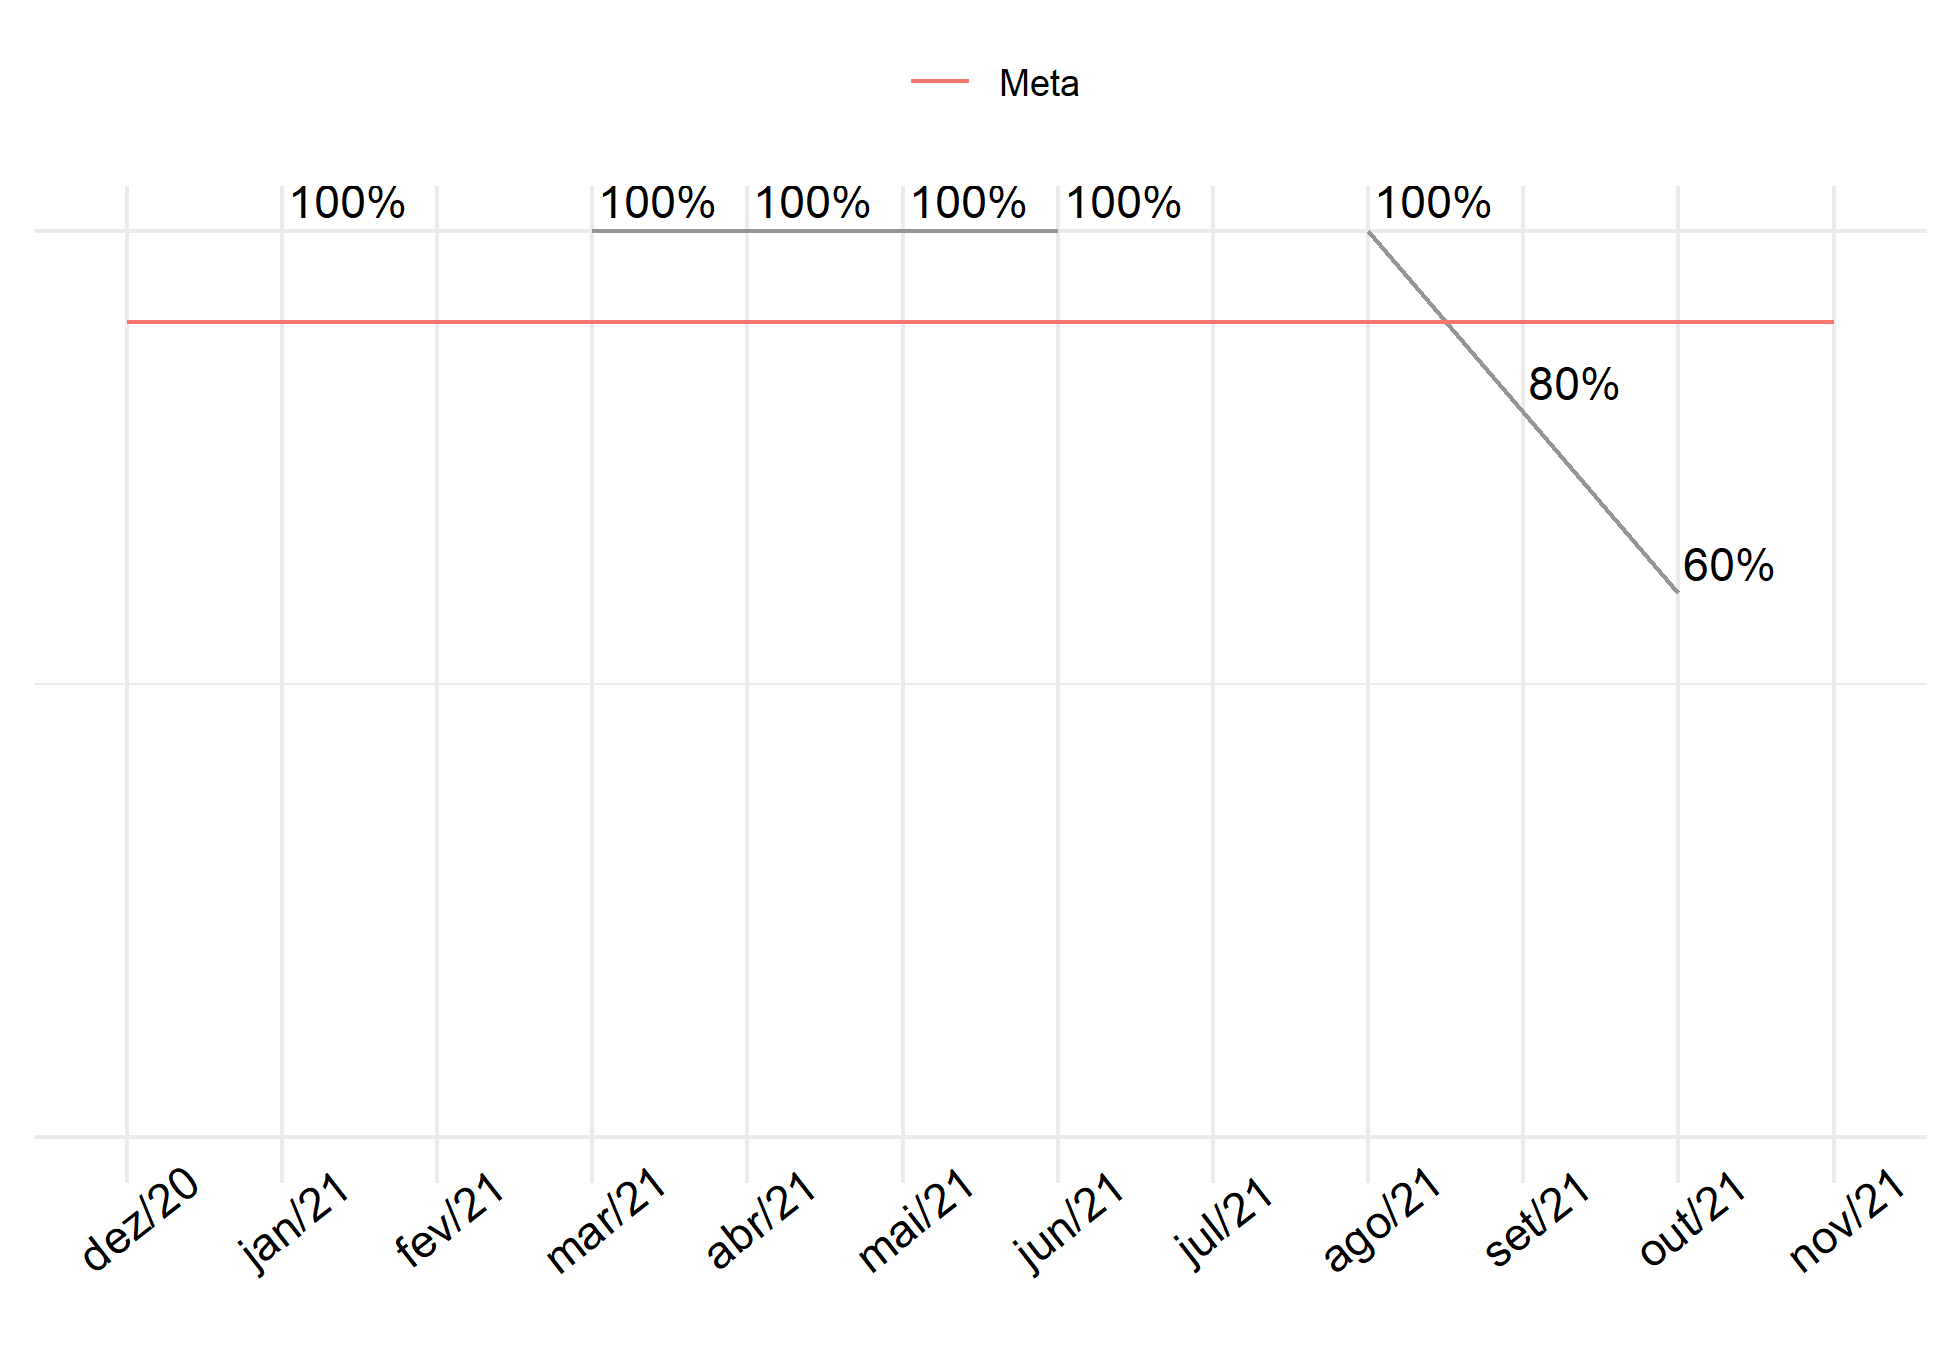
\includegraphics[width=0.7\textwidth]{Imagens/pulseiras.png}
\end{figure}

\begin{center}
 \textbf{Meta: 90\%}
\end{center}

\begin{figure}[H]
\caption{Proporção de criados identificados entre os criados observados, programas de internação}
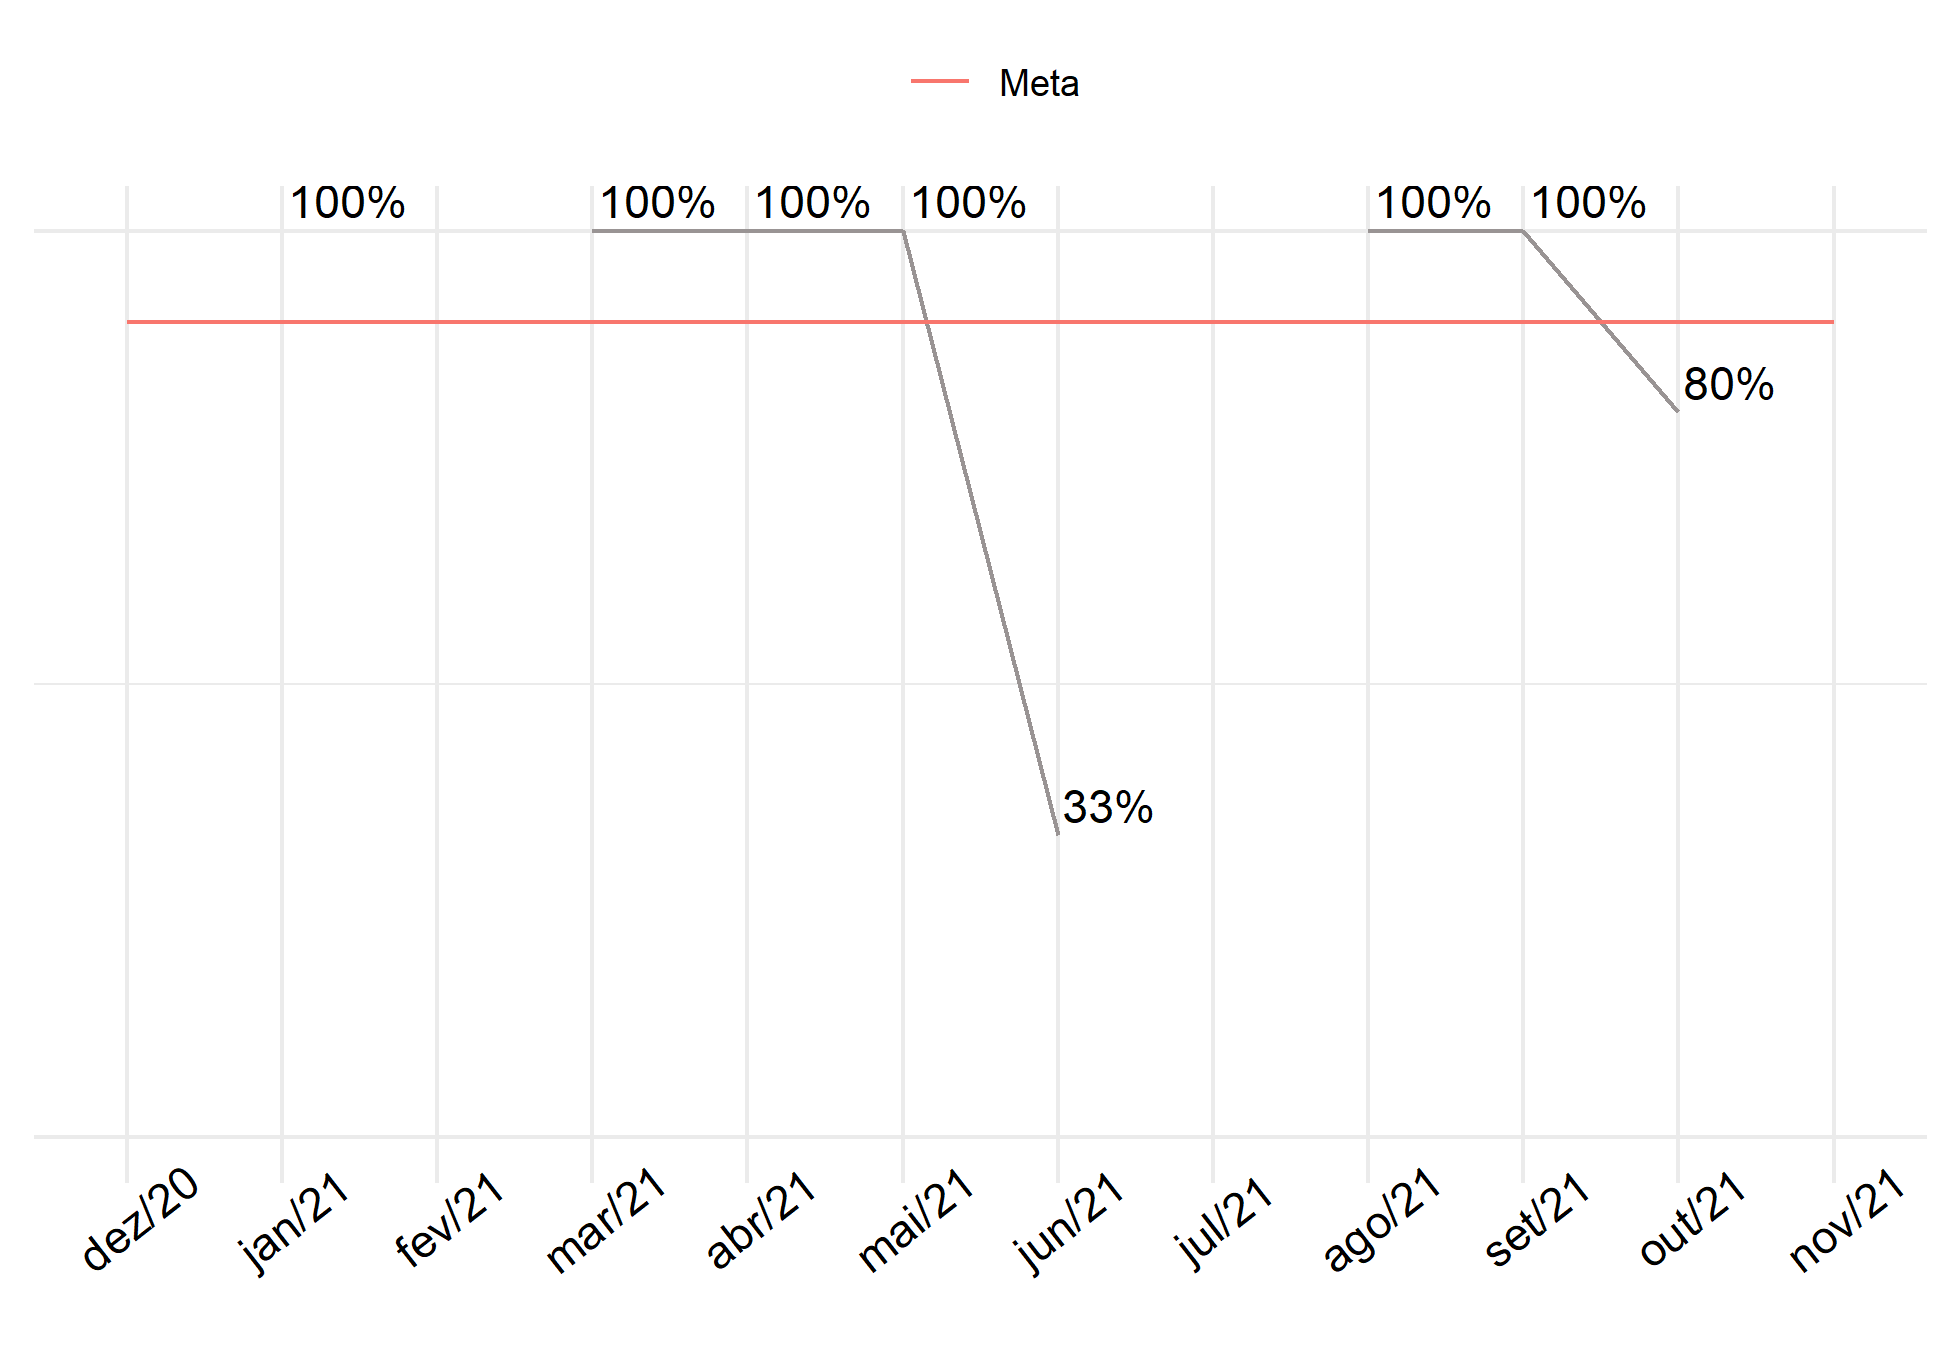
\includegraphics[width=0.7\textwidth]{Imagens/criado.png}
\end{figure}

\begin{center}
 \textbf{Meta: 100\%}
\end{center}

\begin{figure}[H]
\caption{Proporção de cama-macas identificadas entre as cama-macas observadas, programas de internação}
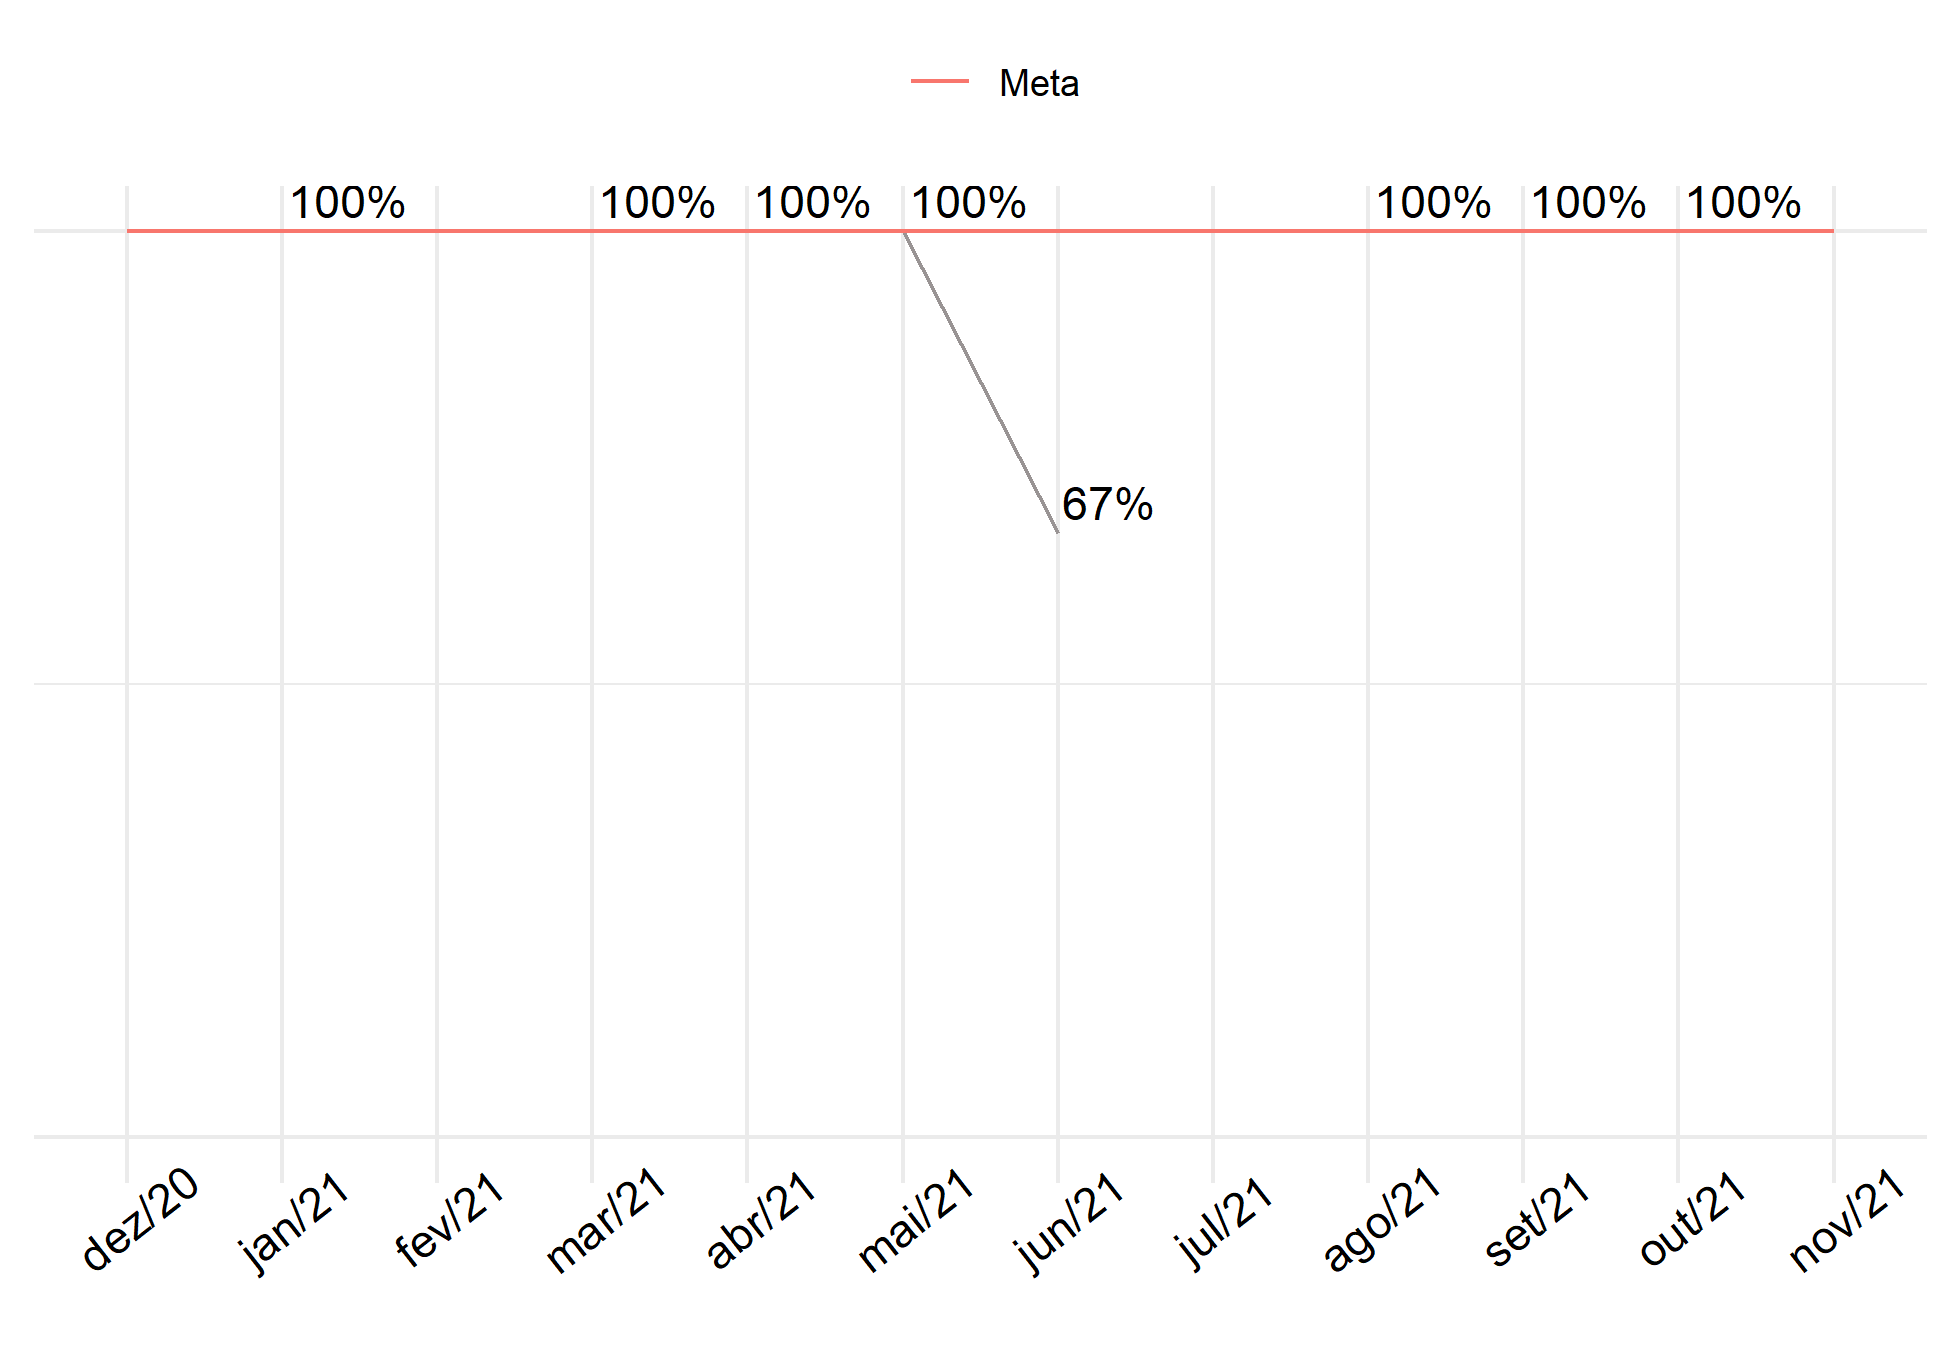
\includegraphics[width=0.7\textwidth]{Imagens/cama.png}
\end{figure}

\begin{center}
 \textbf{Meta: 100\%}
\end{center}

\newpage

\subsection{Meta 2 – Melhorar a Comunicação entre os Profissionais de Saúde}

\subsubsection{Indicador de Estrutura}

Protocolo de Comunicação Segura implantado, atualizado e disponível para
as equipes assistenciais. Sistema de Informação Hospitalar, Prontuário
Eletrônico e Sistema de Enfermarias.

\subsubsection{Indicadores de Processo}

Os indicadores de processo em Comunicação Segura representam a adesão ao
repasse seguro de informações nas admissões e altas dos pacientes do
Primeiro Estágio.

\begin{figure}[H]
\caption{Percentual de preenchimento do check list de comunicação segura à admissão, 1° Estágio}
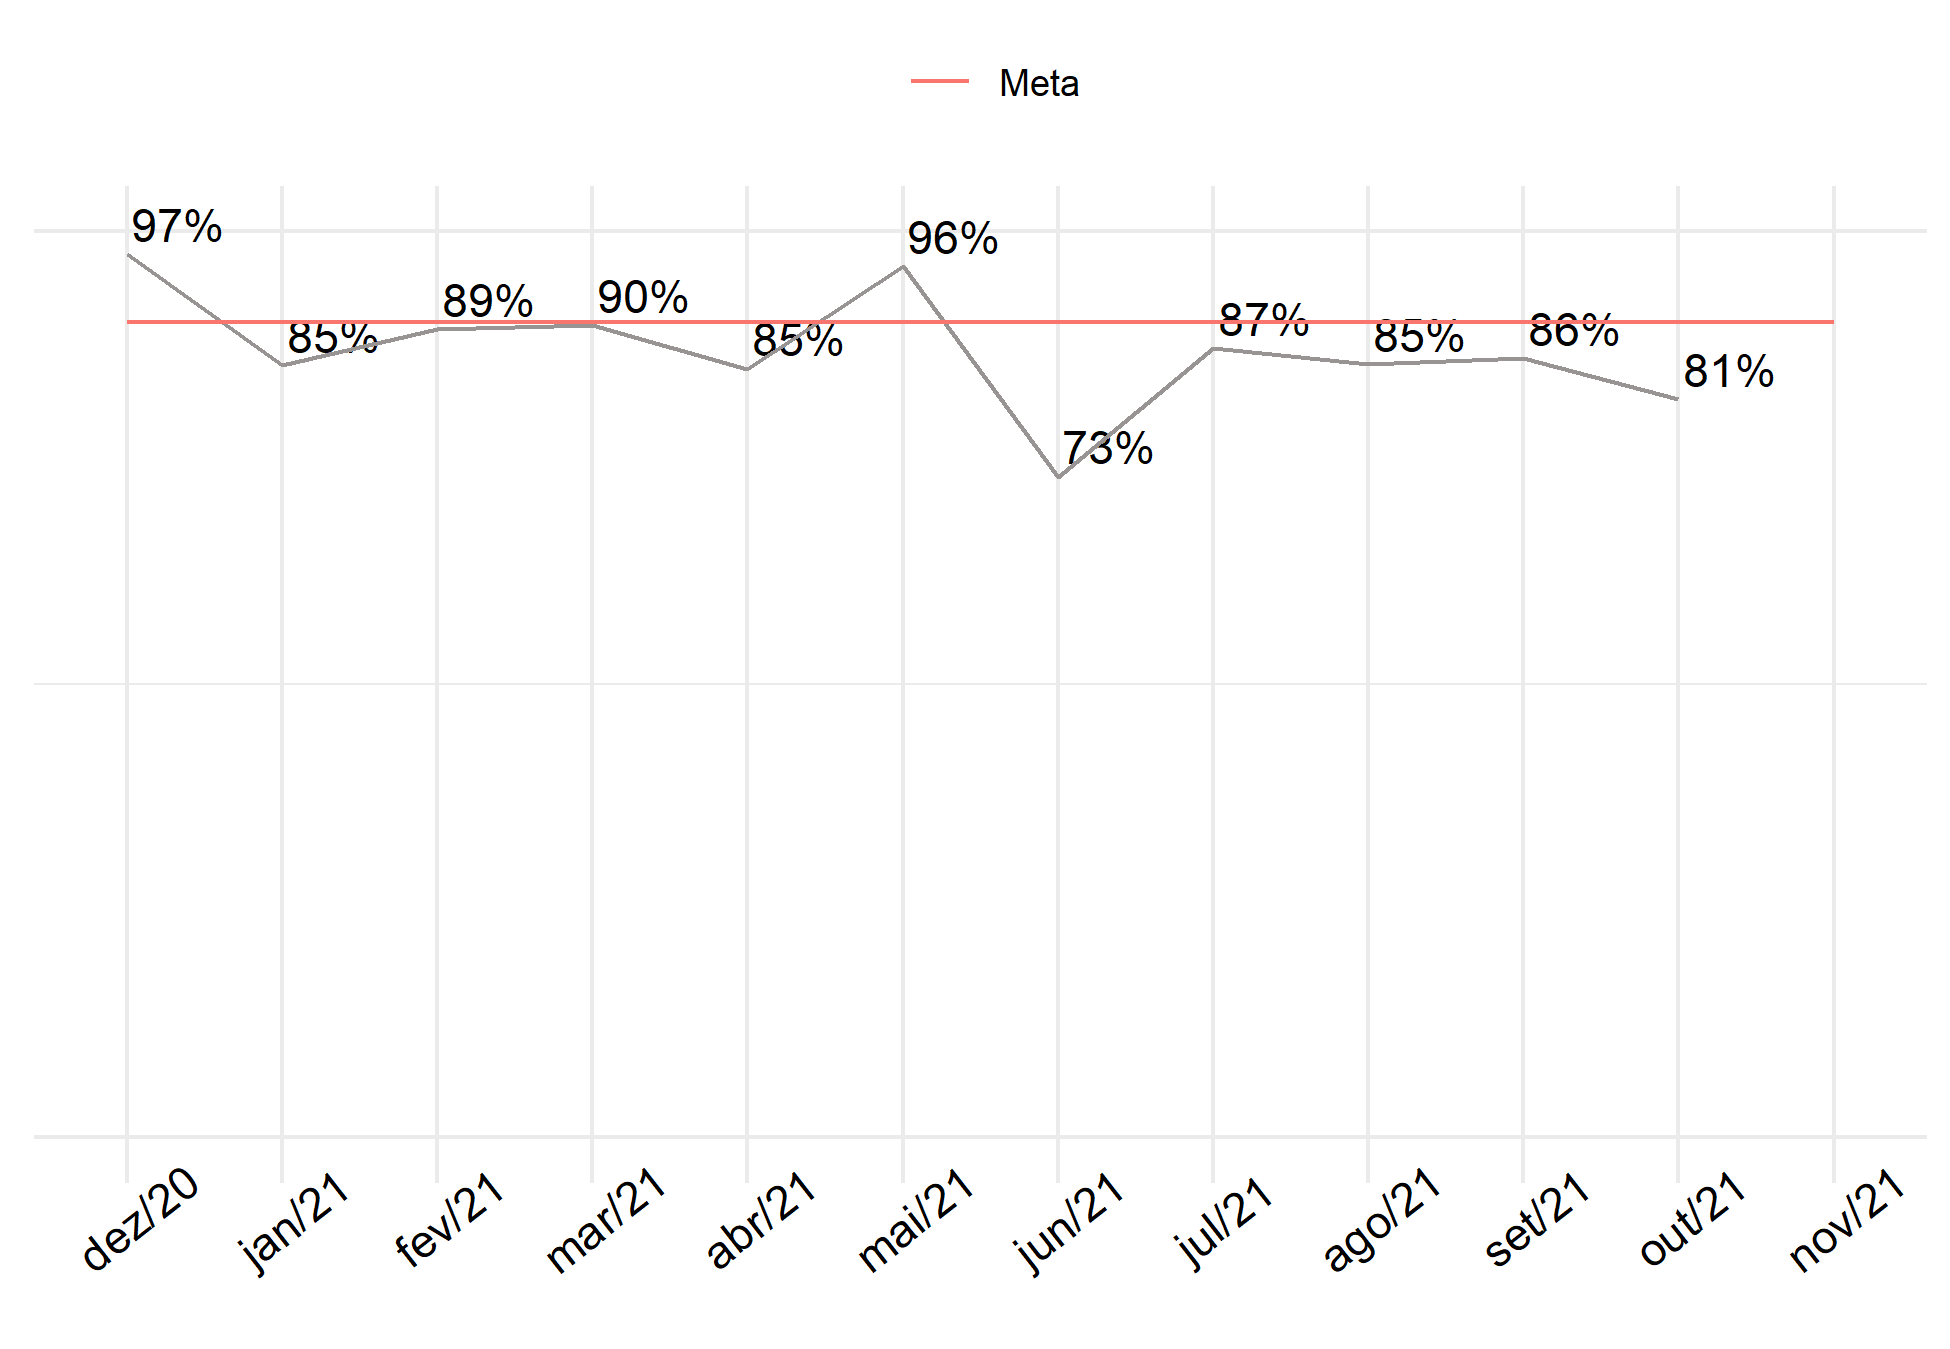
\includegraphics[width=0.7\textwidth]{Imagens/check_admissao.png}
\end{figure}

\begin{center}
 \textbf{Meta: 90\%}
\end{center}

\begin{figure}[H]
\caption{Percentual de preenchimento do check list de comunicação segura na alta, 1° Estágio}
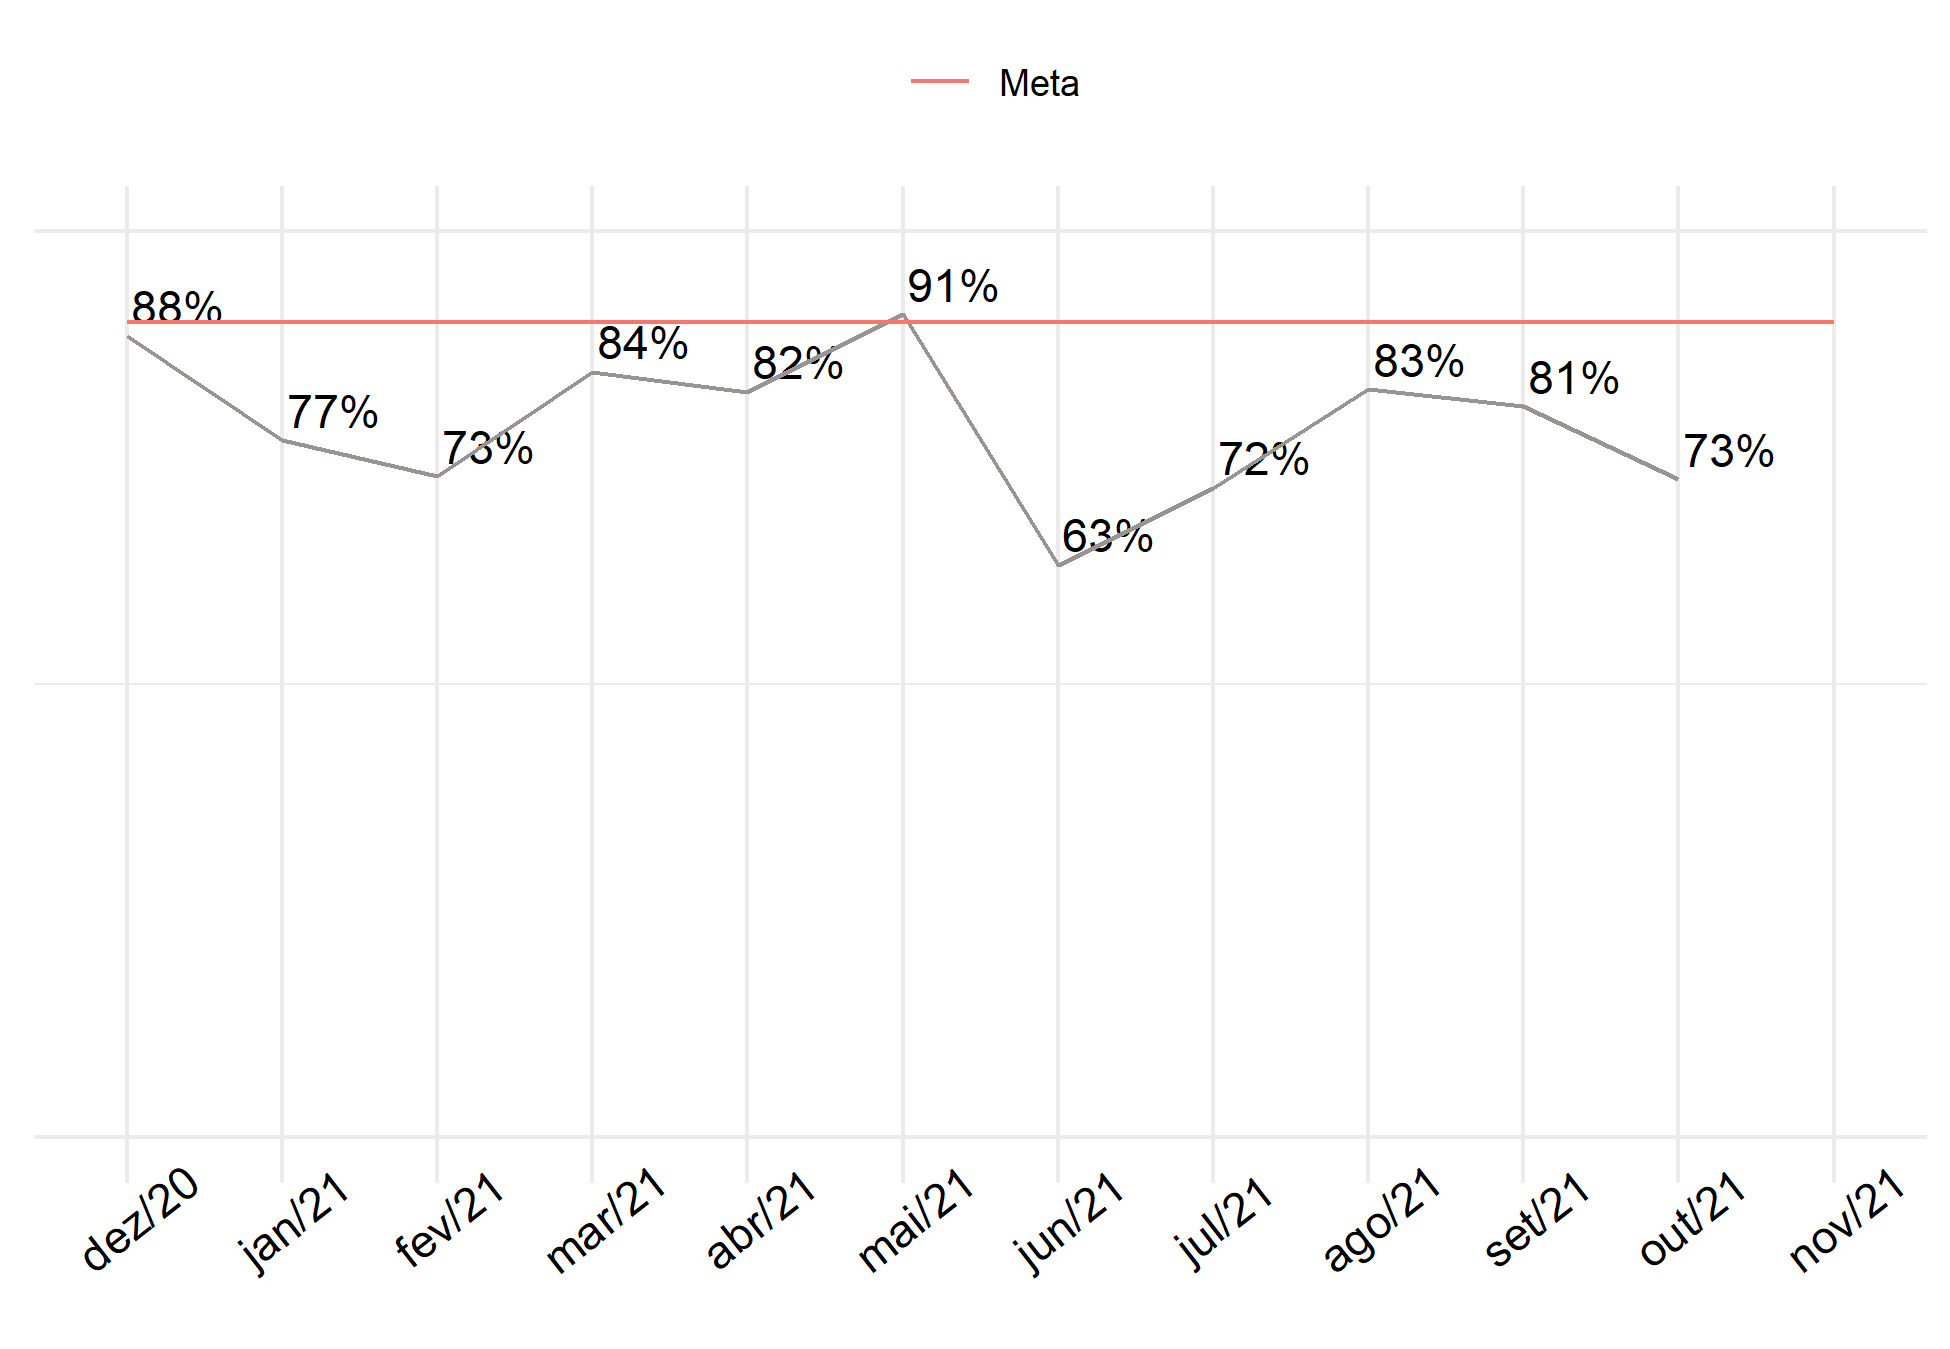
\includegraphics[width=0.7\textwidth]{Imagens/check_alta.png}
\end{figure}

\begin{center}
 \textbf{Meta: 90\%}
\end{center}

\subsection{Meta 3 – Melhorar a Segurança na Prescrição, Dispensação e Administração de Medicamentos}

\subsubsection{Indicador de Estrutura}

Protocolo de Segurança na Prescrição, Dispensação e Administração de
Medicamentos implantado, atualizado e divulgado para as equipes
assistenciais.

\subsubsection{Indicadores de Resultado}

Os indicadores representam as informações referentes aos programas de
internação.

\begin{figure}[H]
\caption{Taxa de erros na prescrição de medicamentos, programas de internação}
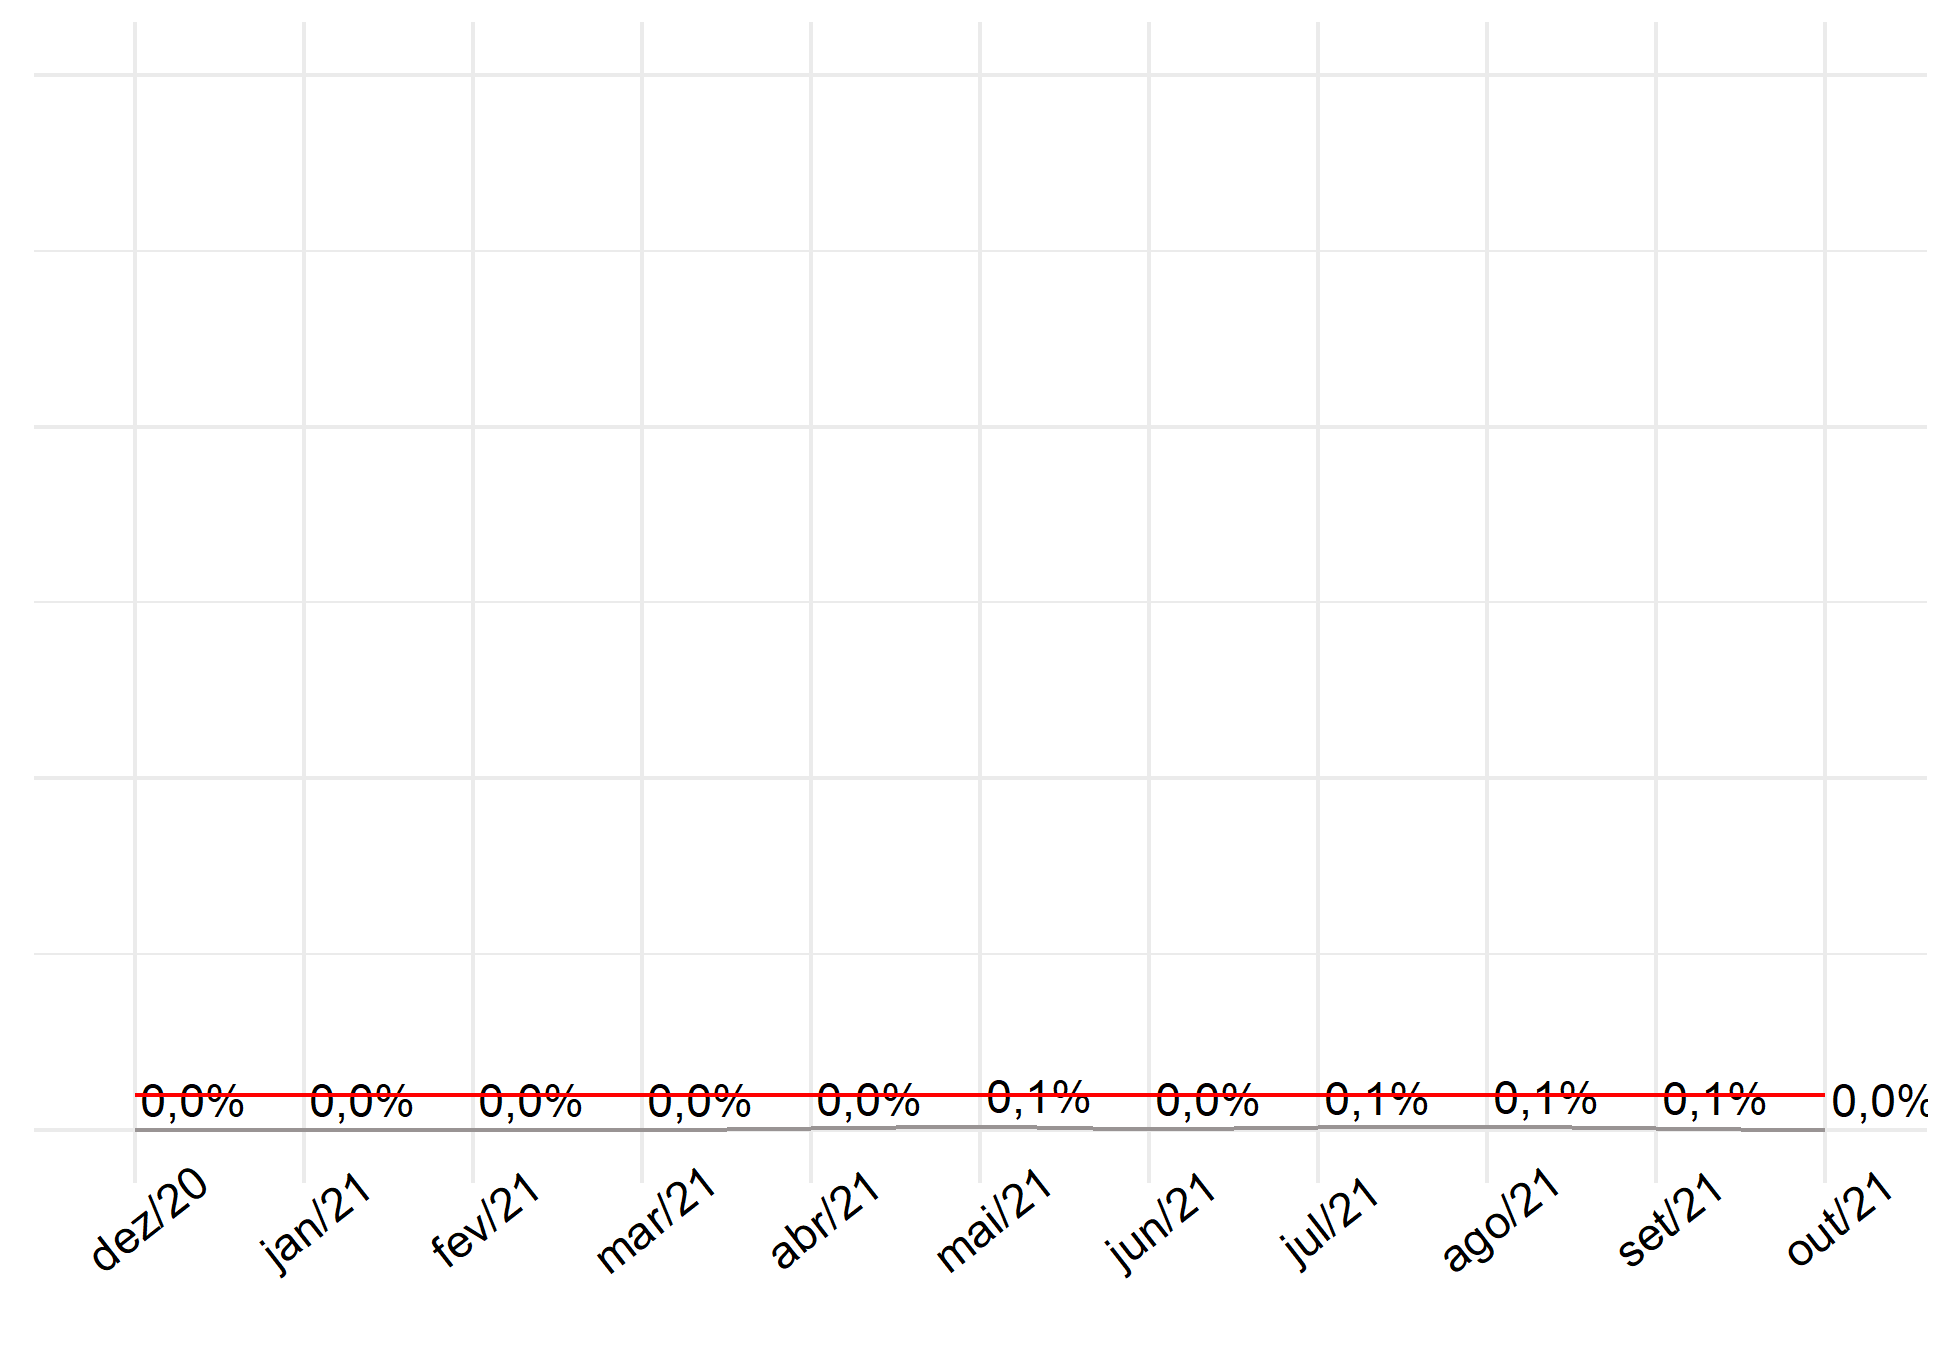
\includegraphics[width=0.7\textwidth]{Imagens/med_prescritos.png}
\end{figure}

\begin{center}
 \textbf{Meta: máximo aceitavel de 1\%}
\end{center}

\begin{figure}[H]
\caption{Taxa de erros na dispensação de medicamentos, programas de internação}
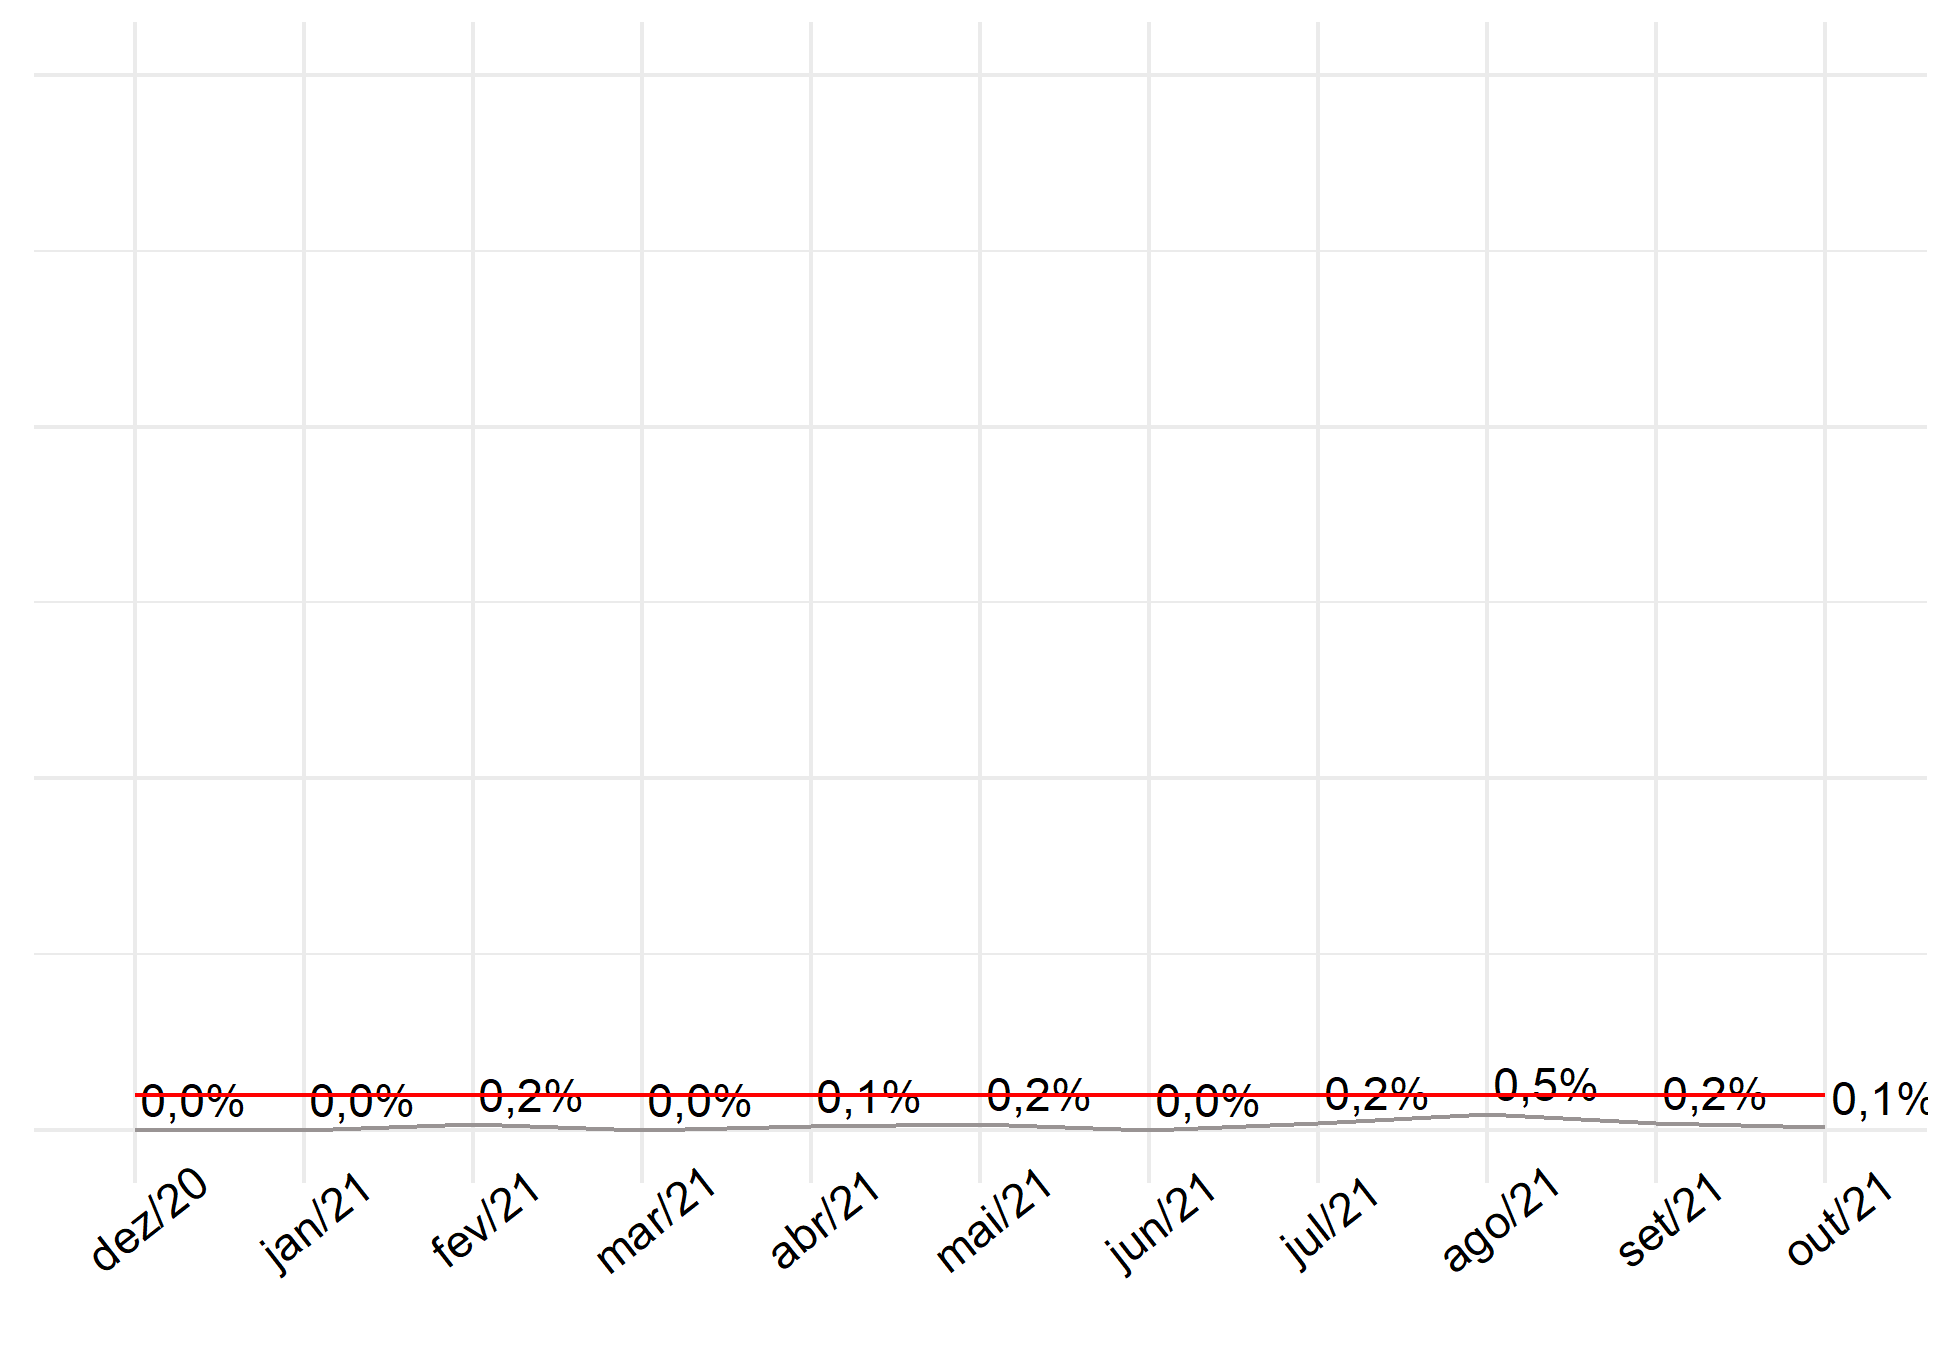
\includegraphics[width=0.7\textwidth]{Imagens/med_dispensados.png}
\end{figure}

\begin{center}
 \textbf{Meta: máximo aceitavel de 1\%}
\end{center}

\subsection{Meta 4 – Assegurar a cirurgia em local de intervenção, procedimento e paciente corretos}

\subsubsection{PROTOCOLO DE CIRURGIA SEGURA}

\textbf{INDICADORES DE ESTRUTURA}

Protocolo de Cirurgia Segura implantado, atualizado e divulgado para as
equipes assistenciais.

\hspace{1cm} O Protocolo de Cirurgia Segura integra as recomendações da
RDC nº 36 de 25 de Julho de 2013 e compõe o Anexo 2 da Portaria nº 1.377
de 24 de julho de 2013. As medidas propostas objetivam a redução de
incidentes e eventos adversos, além de assegurar a realização de
procedimentos cirúrgicos no local e no paciente correto.

\hspace{1cm} Os indicadores em destaque no Plano de Segurança do
Paciente da Rede SARAH para este protocolo são:

\textbf{INDICADORES DE RESULTADO}

\begin{table}[H]

\caption{\label{tab:unnamed-chunk-11}Número de cirurgias em paciente errado, programas de internação}
\centering
\resizebox{\linewidth}{!}{
\begin{tabular}[t]{lrrrrrrrrrrrrr}
\toprule
 & dez/20 & jan/21 & fev/21 & mar/21 & abr/21 & mai/21 & jun/21 & jul/21 & ago/21 & set/21 & out/21 & nov/21 & Total\\
\midrule
Evento Adverso & 0 & 0 & 0 & 0 & 0 & 0 & 0 & 0 & 0 & 0 & 0 & 0 & 0\\
\midrule
\textbf{Total} & \textbf{0} & \textbf{0} & \textbf{0} & \textbf{0} & \textbf{0} & \textbf{0} & \textbf{0} & \textbf{0} & \textbf{0} & \textbf{0} & \textbf{0} & \textbf{0} & \textbf{0}\\
\bottomrule
\end{tabular}}
\end{table}

\begin{table}[H]

\caption{\label{tab:unnamed-chunk-12}Número de cirurgias em local errado, programas de internação}
\centering
\resizebox{\linewidth}{!}{
\begin{tabular}[t]{lrrrrrrrrrrrrr}
\toprule
 & dez/20 & jan/21 & fev/21 & mar/21 & abr/21 & mai/21 & jun/21 & jul/21 & ago/21 & set/21 & out/21 & nov/21 & Total\\
\midrule
Evento Adverso & 0 & 0 & 0 & 0 & 0 & 0 & 0 & 0 & 0 & 0 & 0 & 0 & 0\\
\midrule
\textbf{Total} & \textbf{0} & \textbf{0} & \textbf{0} & \textbf{0} & \textbf{0} & \textbf{0} & \textbf{0} & \textbf{0} & \textbf{0} & \textbf{0} & \textbf{0} & \textbf{0} & \textbf{0}\\
\bottomrule
\end{tabular}}
\end{table}

\begin{table}[H]

\caption{\label{tab:unnamed-chunk-13}Número de procedimentos cirúrgicos errados, programas de internação}
\centering
\resizebox{\linewidth}{!}{
\begin{tabular}[t]{lrrrrrrrrrrrrr}
\toprule
 & dez/20 & jan/21 & fev/21 & mar/21 & abr/21 & mai/21 & jun/21 & jul/21 & ago/21 & set/21 & out/21 & nov/21 & Total\\
\midrule
Evento Adverso & 0 & 0 & 0 & 0 & 0 & 0 & 0 & 0 & 0 & 0 & 0 & 0 & 0\\
\midrule
\textbf{Total} & \textbf{0} & \textbf{0} & \textbf{0} & \textbf{0} & \textbf{0} & \textbf{0} & \textbf{0} & \textbf{0} & \textbf{0} & \textbf{0} & \textbf{0} & \textbf{0} & \textbf{0}\\
\bottomrule
\end{tabular}}
\end{table}

\textbf{INDICADOR DE PROCESSO}

\hspace{1cm} As melhores práticas recomendam o uso de da Lista de
Verificação da Cirurgia Segura. Esta deve ser aplicada por um único
condutor, nos seguintes momentos do ato operatório: 1) antes da indução
anestésica; 2) antes da incisão cirúrgica e, 3) antes do paciente sair
da sala de cirurgia. O indicador proposto pelo Plano de Segurança da
Rede SARAH para o monitoramento desta atividade está representado
abaixo:

\begin{figure}[H]
\caption{Taxa de adesão à Lista de Verificação da Cirurgia Segura}
\includegraphics[width=0.7\textwidth]{Imagens/lista_verificacao_centro_cirurgico.png}
\end{figure}

\begin{center}
 \textbf{Meta: 95\%}
\end{center}

\subsection{PROTOCOLO DE PREVENÇÃO DE INFECÇÃO DO SÍTIO CIRÚRGICO}

\hspace{1cm} O Protocolo de Prevenção de Infecção Relacionada à
Assistência (IRAS) integra as recomendações da RDC nº 36 de 25 de Julho
de 2013 sendo a Prevenção da Infecção do Sítio Cirúrgico (ICS) uma das
circunstâncias elegíveis. O monitoramento deste Protocolo se dará
mediante o acompanhamento dos seguintes indicadores:

\begin{figure}[H]
\caption{Taxa de antibiótico profilático administrado 30 a 60 minutos antes da incisão}
\includegraphics[width=0.7\textwidth]{Imagens/profilaxia30-60_centro_cirurgico.png}
\end{figure}

\begin{center}
 \textbf{Meta: 90\%}
\end{center}

\begin{figure}[H]
\caption{Taxa de duração do antibiótico profilático em até 24 horas}
\includegraphics[width=0.7\textwidth]{Imagens/profilaxia_ate_24h_centro_cirurgico.png}
\end{figure}

\begin{center}
 \textbf{Meta: 90\%}
\end{center}

\begin{figure}[H]
\caption{Taxa tricotomia com intervalo menor ou igual a 2h}
\includegraphics[width=0.7\textwidth]{Imagens/tricotomia_centro_cirurgico.png}
\end{figure}

\begin{center}
 \textbf{Meta: 90\%}
\end{center}

\newpage

\subsection{PROTOCOLO DE PREVENÇÃO DE LESÃO POR PRESSÃO}

\hspace{1cm} O Protocolo de Prevenção de Lesão por Pressão compõe a RCD
nº 36 de julho de 2013 estando as ações descritas no anexo 1 da Portaria
nº 1.377 de 9 de julho 2013 / Ministério da Saúde. As recomendações
envolvem a estratificação do risco para lesões por pressão à admissão e
adoção de medidas preventivas conforme o risco. O monitoramento deste
protocolo se fará mediante o acompanhamento dos seguintes indicadores:

\begin{figure}[H]
\caption{Percentual de pacientes com tempo de posicionamento cirúrgico até 3h e que desenvolveram Lesão por Pressão}
\includegraphics[width=0.7\textwidth]{Imagens/lesao_pressao_centro_cirurgico.png}
\end{figure}

\newpage
\subsection{Meta 5 -  Higienizar as mãos para evitar infecções}

\subsubsection{Indicador de Estrutura}

Protocolo de Higienização das Mãos implantado, atualizado e divulgado
para as equipes assistenciais.

\subsubsection{Indicadores de Resultado}

O indicador representa os dados dos programas de internação.

\begin{figure}[H]
\caption{Consumo de preparação alcoólica (ml) por paciente-dia, programas de internação}
\includegraphics[width=0.7\textwidth]{Imagens/higienizacao.png}
\end{figure}

\begin{center}
 \textbf{Meta: 20 ml por paciente-dia}
\end{center}

\subsection{Meta 6 – Reduzir o Risco de Quedas}

\subsubsection{Indicador de Estrutura}

Protocolo de Prevenção de Quedas implantado, atualizado e divulgado para
as equipes assistenciais.

\subsubsection{Indicadores de Processo}

O indicador representa os dados dos programas de Neurorreabilitação e
Ortopedia Infantil, Neurocirurgia/Oncologia, Ortopedia Adulto e
Reabilitação Neurológica.

\begin{figure}[H]
\caption{Proporção de pacientes submetidos à avaliação do risco de queda à admissão}
\includegraphics[width=0.7\textwidth]{Imagens/riscos.png}
\end{figure}

\begin{center}
 \textbf{Meta: 90\%}
\end{center}

\subsubsection{Indicadores de Resultado}

\begin{figure}[H]
\caption{Taxa de quedas por mil pacientes-dia, programas de internação}
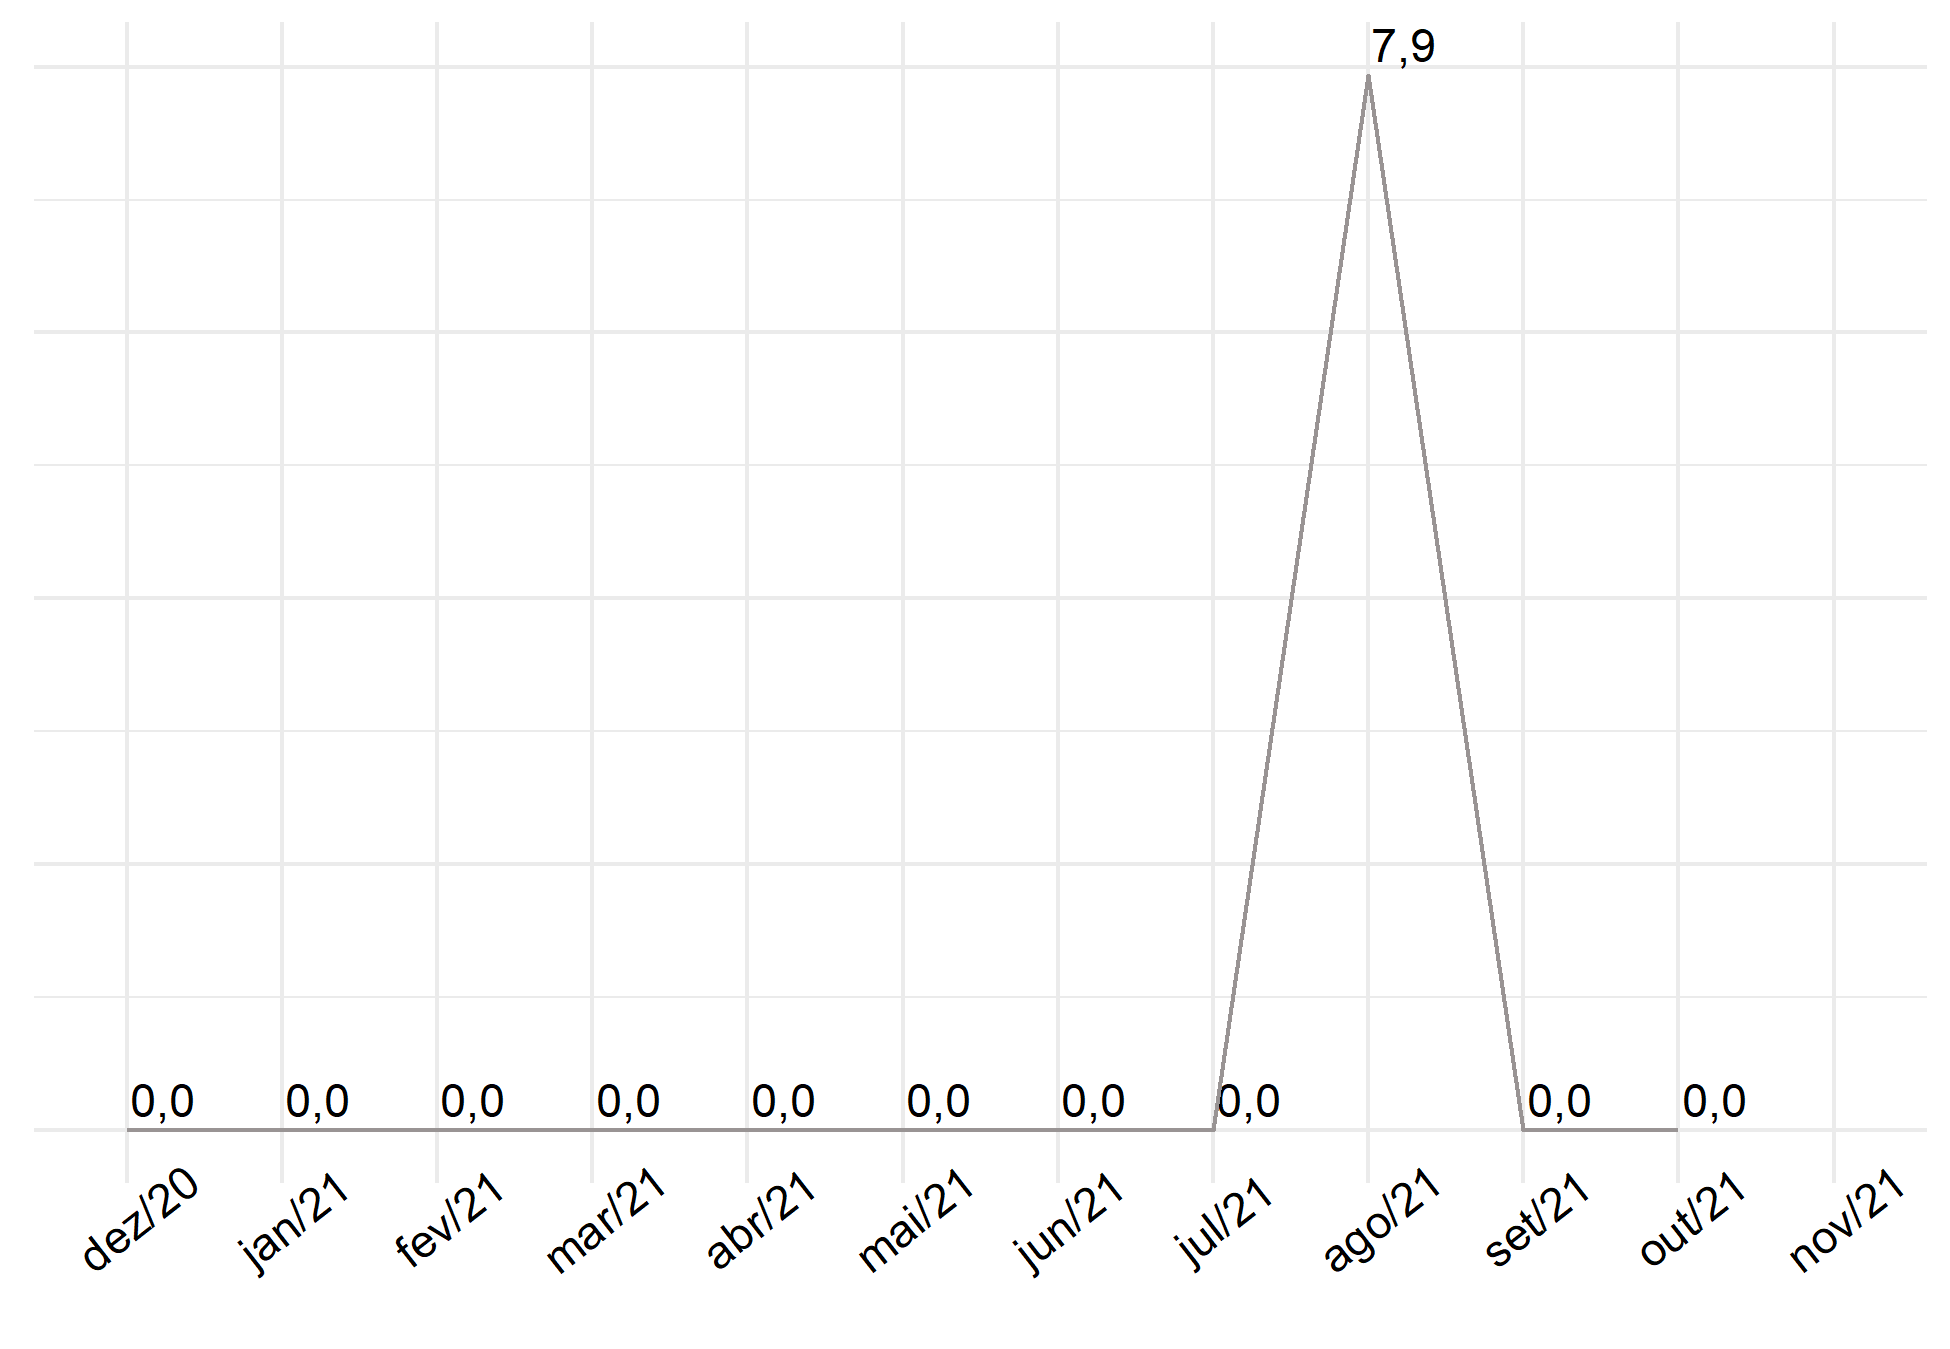
\includegraphics[width=0.7\textwidth]{Imagens/quedas_pacientes_dia.png}
\end{figure}

\begin{figure}[H]
\caption{Taxa de quedas com dano por mil pacientes-dia, programas de internação}
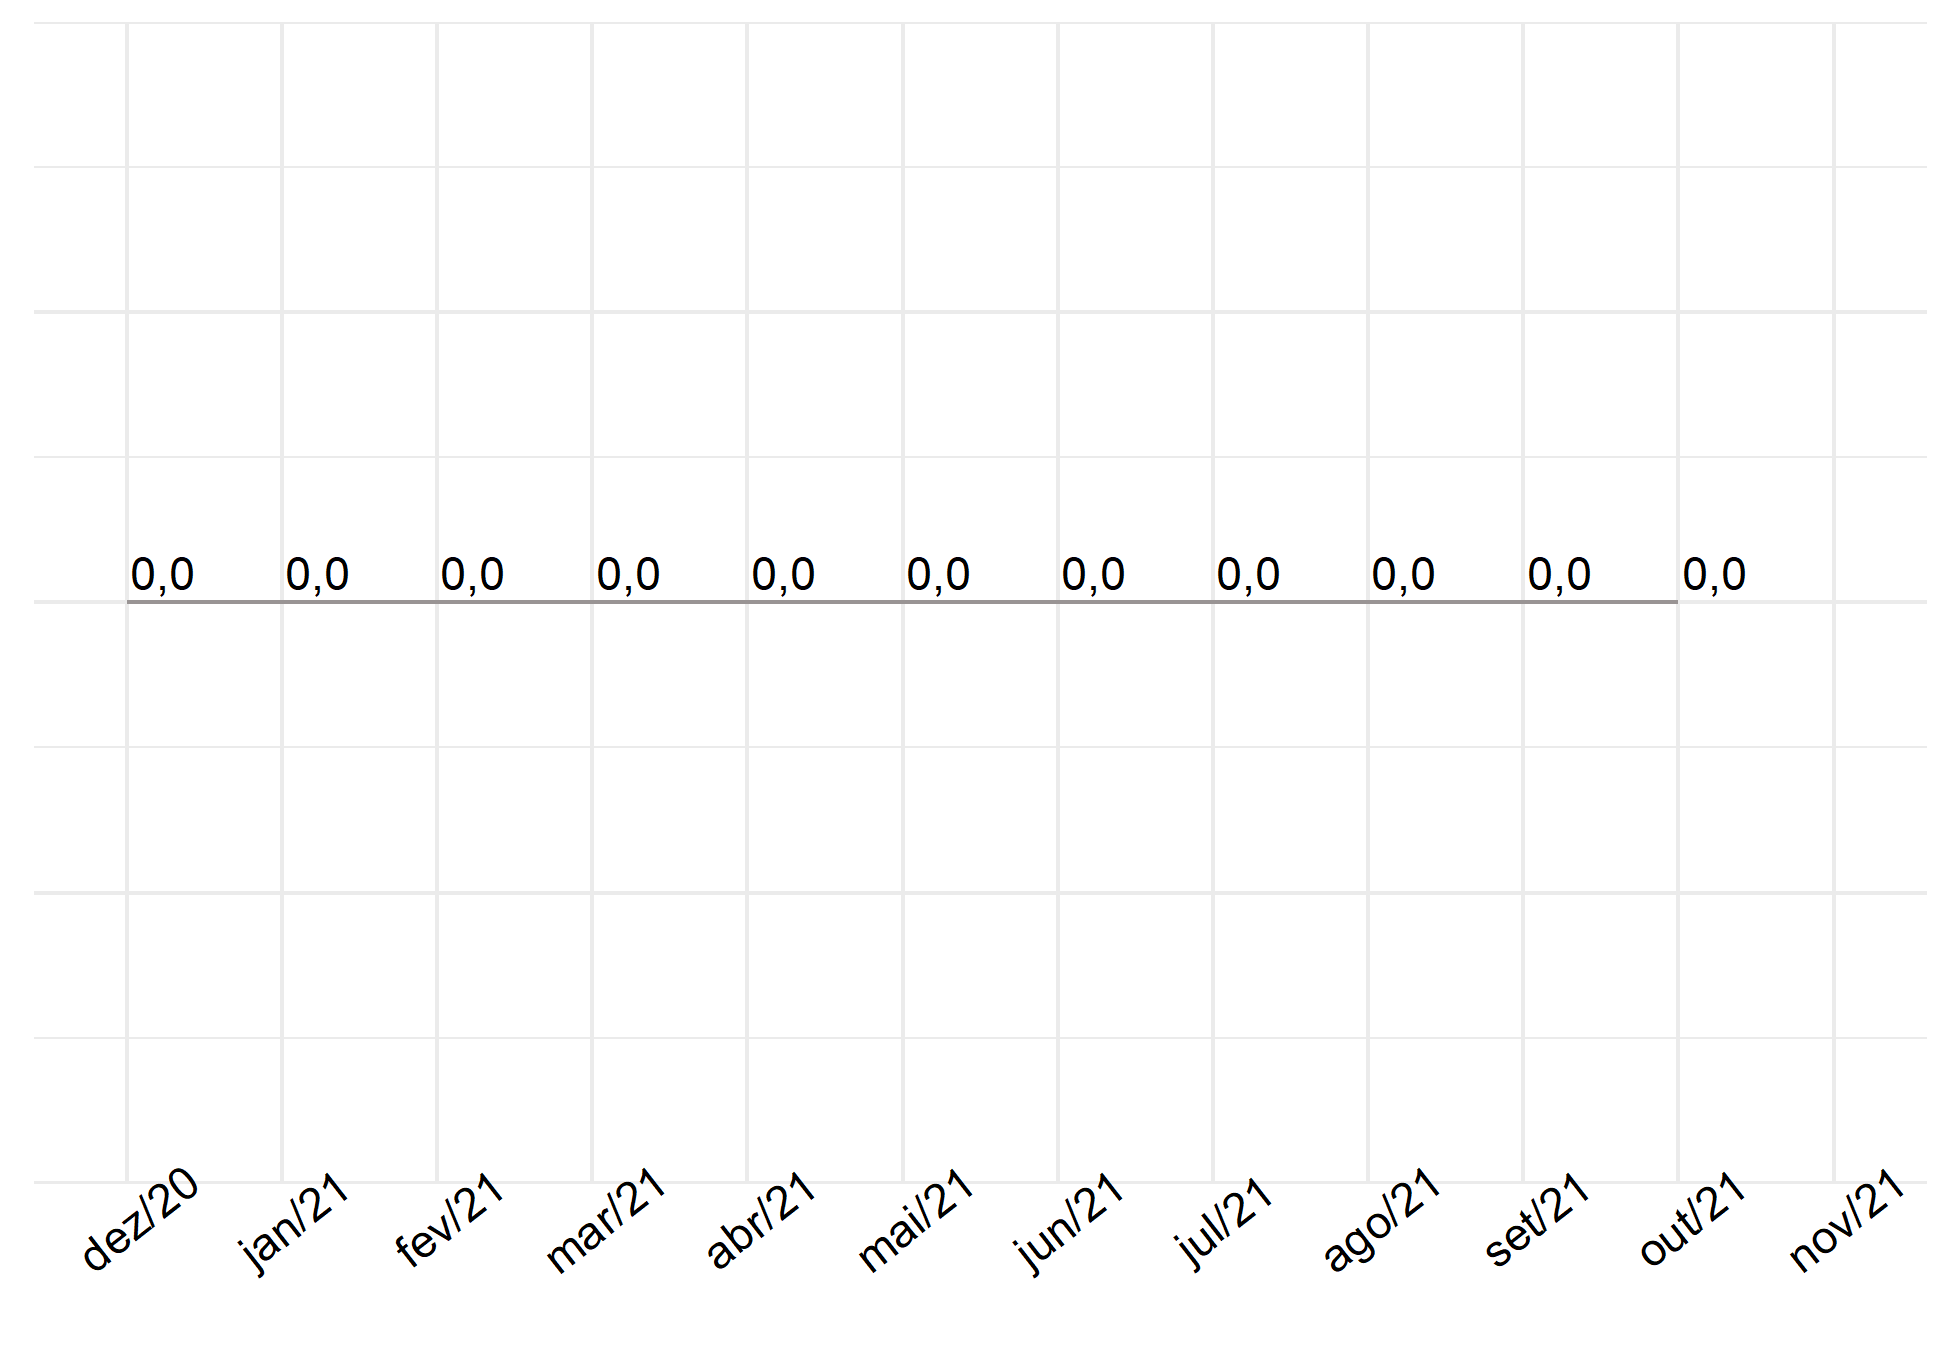
\includegraphics[width=0.7\textwidth]{Imagens/queda_pacientes_dia.png}
\end{figure}

\begin{table}[H]

\caption{\label{tab:unnamed-chunk-24}Distribuição do número de quedas, programas de internação}
\centering
\resizebox{\linewidth}{!}{
\begin{tabular}[t]{lrrrrrrrrrrrrr}
\toprule
 & dez/20 & jan/21 & fev/21 & mar/21 & abr/21 & mai/21 & jun/21 & jul/21 & ago/21 & set/21 & out/21 & nov/21 & Total\\
\midrule
Evento Adverso & 1 & 1 & 1 & 6 & 1 & 1 & 1 & 0 & 3 & 0 & 3 & 0 & 18\\
Incidente sem dano & 13 & 5 & 9 & 5 & 3 & 6 & 9 & 5 & 9 & 5 & 7 & 0 & 76\\
\midrule
\textbf{Total} & \textbf{14} & \textbf{6} & \textbf{10} & \textbf{11} & \textbf{4} & \textbf{7} & \textbf{10} & \textbf{5} & \textbf{12} & \textbf{5} & \textbf{10} & \textbf{0} & \textbf{94}\\
\bottomrule
\end{tabular}}
\end{table}

\begin{table}[H]

\caption{\label{tab:unnamed-chunk-25}Distribuição do número de quedas, demais setores}
\centering
\resizebox{\linewidth}{!}{
\begin{tabular}[t]{lrrrrrrrrrrrrr}
\toprule
 & dez/20 & jan/21 & fev/21 & mar/21 & abr/21 & mai/21 & jun/21 & jul/21 & ago/21 & set/21 & out/21 & nov/21 & Total\\
\midrule
Evento Adverso & 0 & 0 & 1 & 1 & 1 & 0 & 0 & 0 & 1 & 0 & 1 & 0 & 5\\
Incidente sem dano & 1 & 1 & 0 & 0 & 0 & 2 & 1 & 0 & 0 & 1 & 0 & 0 & 6\\
\midrule
\textbf{Total} & \textbf{1} & \textbf{1} & \textbf{1} & \textbf{1} & \textbf{1} & \textbf{2} & \textbf{1} & \textbf{0} & \textbf{1} & \textbf{1} & \textbf{1} & \textbf{0} & \textbf{11}\\
\bottomrule
\end{tabular}}
\end{table}

\subsection{Meta 7 – Prevenir Lesões por Pressão (LPP)}

\subsubsection{Indicador de Estrutura}

Protocolo de Prevenção de Lesão por Pressão implantado, atualizado e
divulgado para as equipes assistenciais.

\subsubsection{Indicadores de Processo}

O indicador representa os dados dos programas de Neurorreabilitação e
Ortopedia Infantil, Neurocirurgia/Oncologia, Ortopedia Adulto e
Reabilitação Neurológica.

\begin{figure}[H]
\caption{Percentual de pacientes submetidos à avaliação do risco de LPP à admissão}
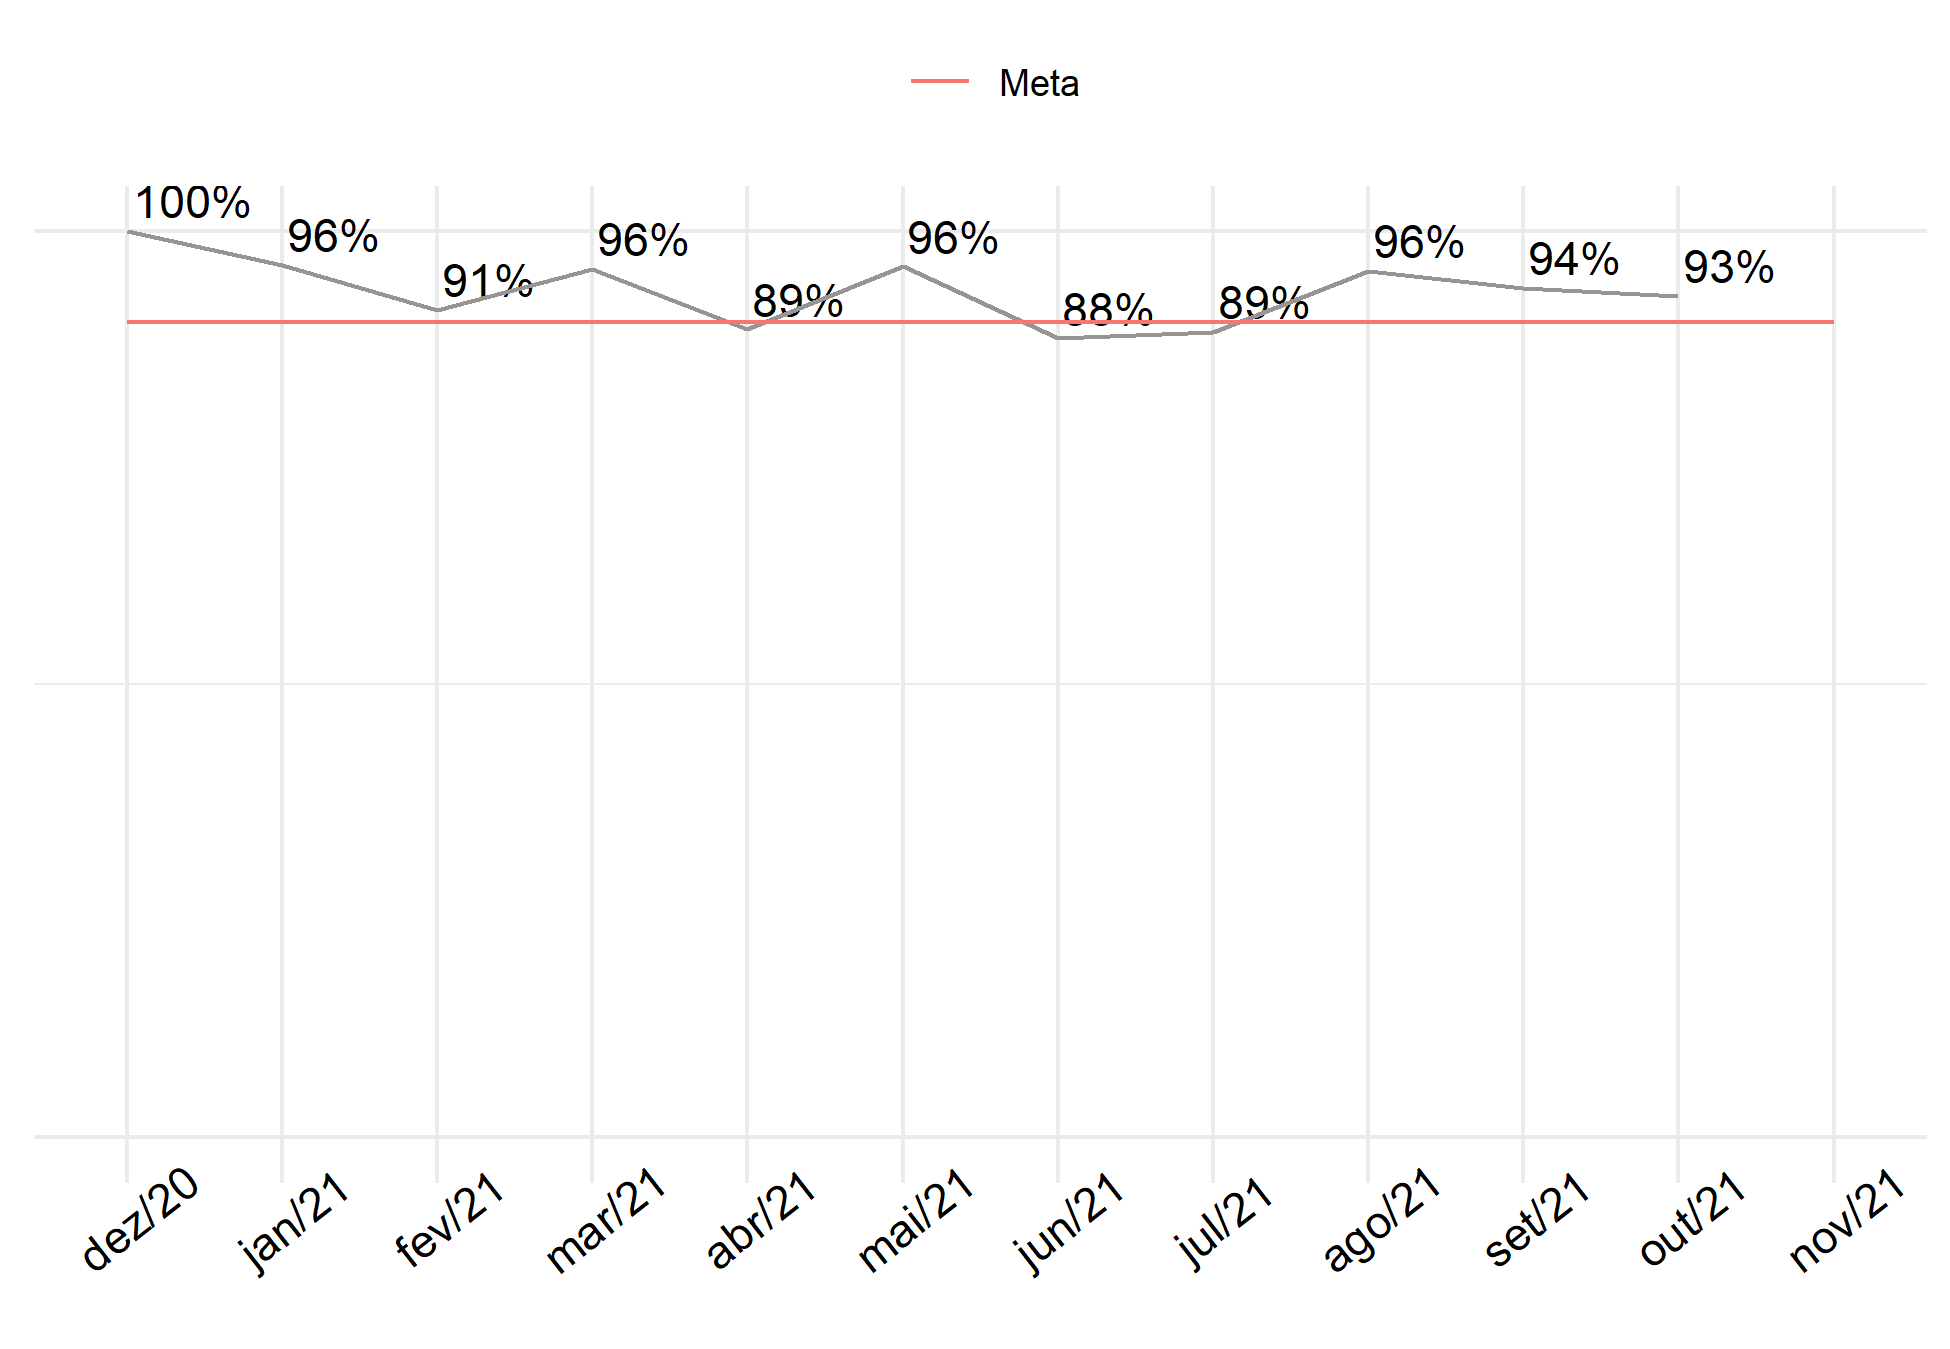
\includegraphics[width=0.7\textwidth]{Imagens/lesao_pressao.png}
\end{figure}

\begin{center}
 \textbf{Meta: 90\%}
\end{center}

O indicador a seguir representa os dados dos programas de internação.

\begin{figure}[H]
\caption{Taxa de Lesão por Pressão por mil pacientes-dia, programas de internação}
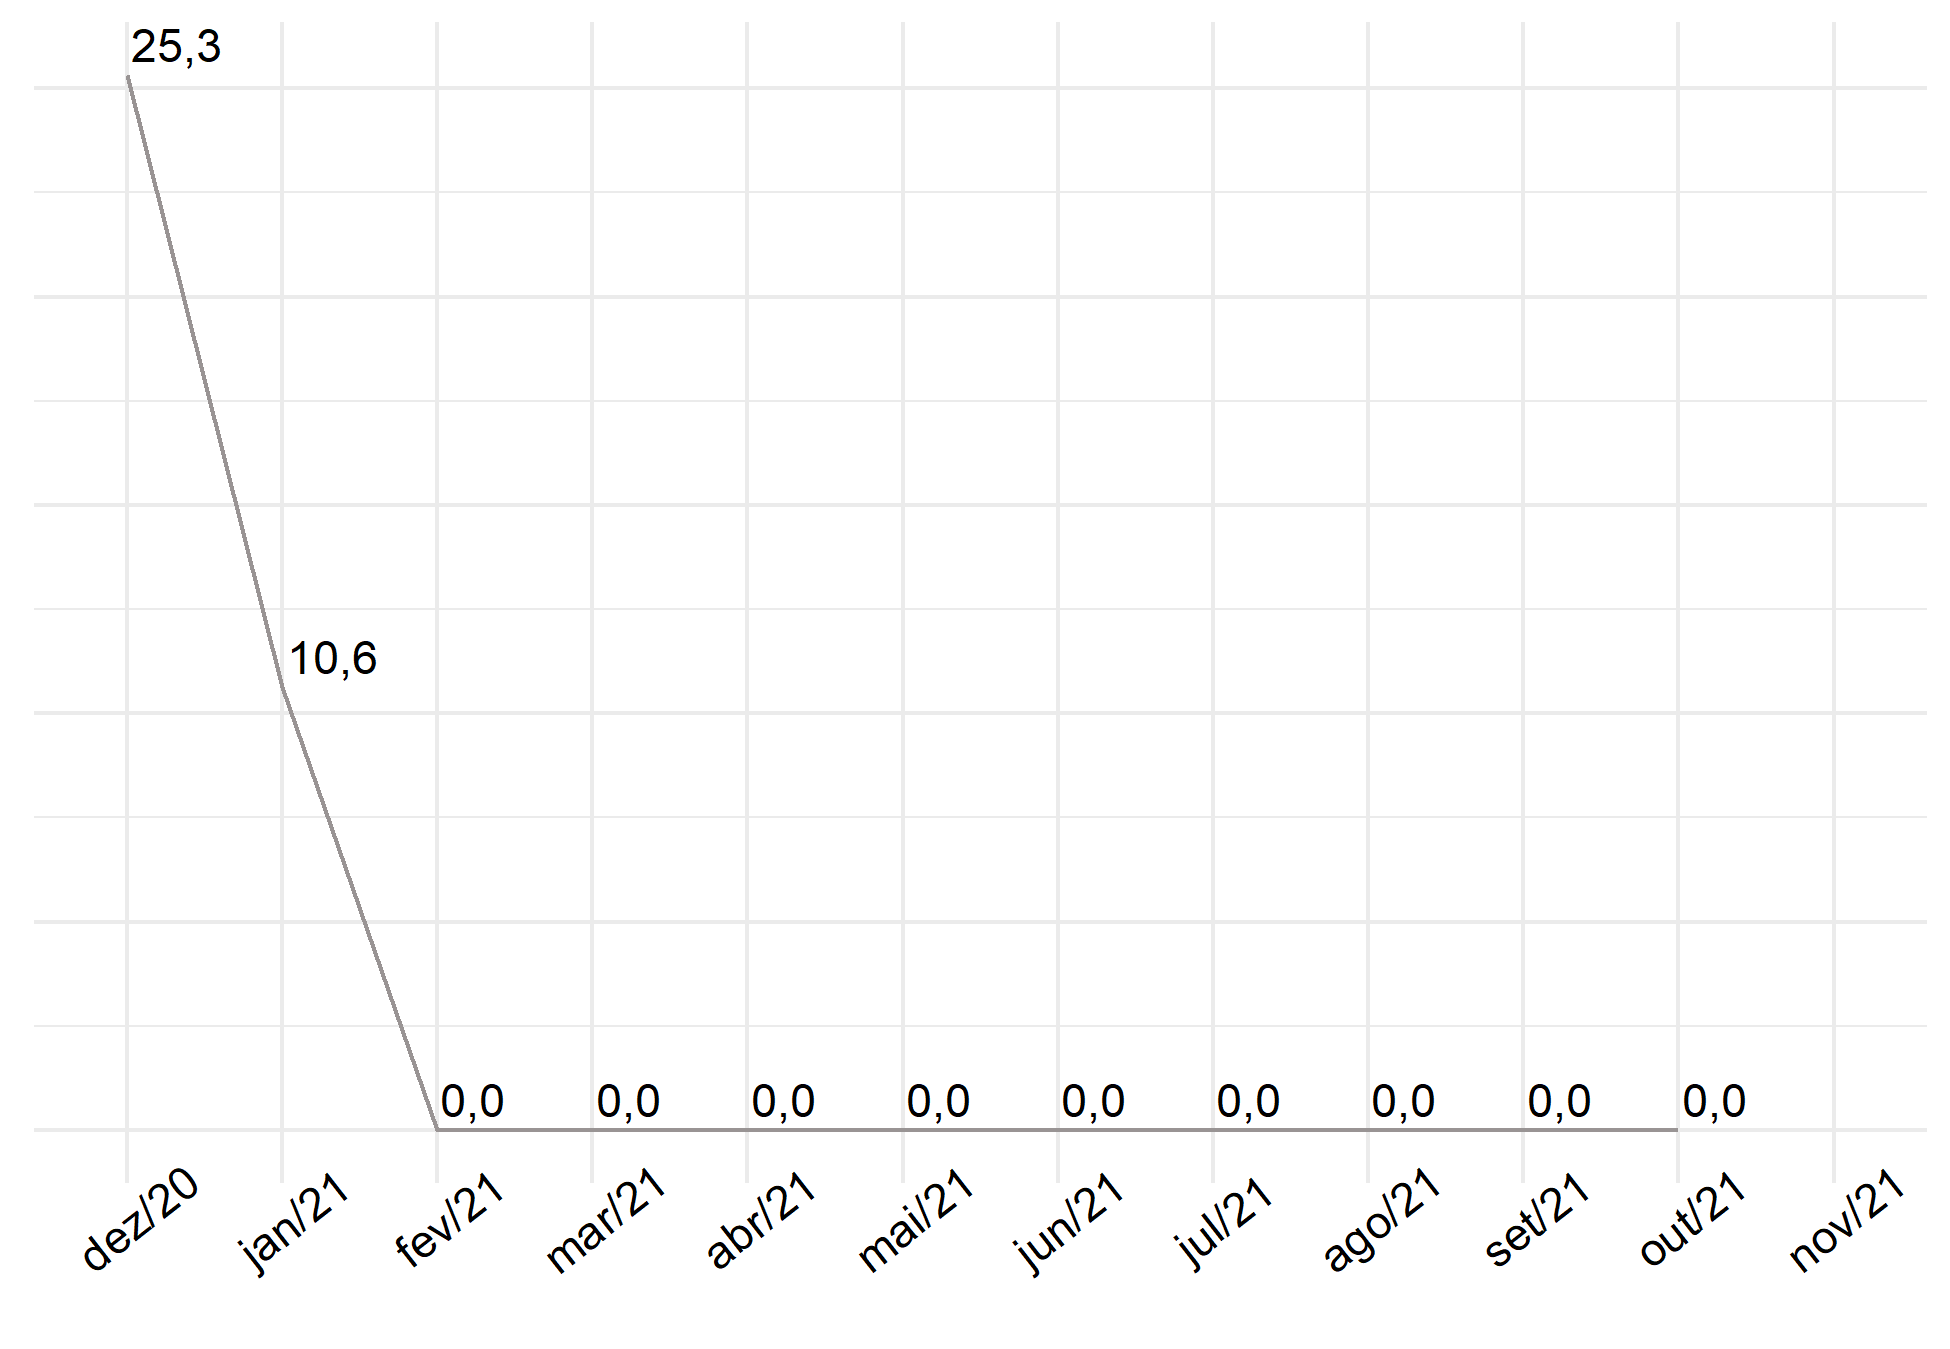
\includegraphics[width=0.7\textwidth]{Imagens/lesaoPressao_pacientes_dia.png}
\end{figure}

\newpage

\subsection{Outros indicadores}

\subsubsection{Indicadores de Processo}

Os indicadores representam os dados dos programas de internação.

\begin{figure}[H]
\caption{Taxa de pacientes triados quanto ao risco nutricional na admissão, programas de internação}
\includegraphics[width=0.7\textwidth]{Imagens/triados.png}
\end{figure}

\begin{figure}[H]
\caption{Prevalência de pacientes admitidos com déficit/risco nutricional *, programas de internação}
\includegraphics[width=0.7\textwidth]{Imagens/prevalencia.png}
\end{figure}

\newpage

\subsubsection{Indicadores de Resultado}

\begin{table}[H]

\caption{\label{tab:unnamed-chunk-31}Incidência de Perda do CNE nos pacientes em TNE, programas de internação}
\centering
\begin{tabu} to \linewidth {>{\raggedright}X>{\raggedright}X>{\raggedright}X>{\raggedright}X>{\raggedright}X>{\raggedright}X>{\raggedright}X>{\raggedright}X>{\raggedright}X>{\raggedright}X>{\raggedright}X>{\raggedright}X}
\toprule
jan & fev & mar & abr & mai & jun & jul & ago & set & out & nov & dez\\
\midrule
0\% & 0\% & 0\% & 0\% & 2\% & 0\% & 0\% & 0\% & 0\% & 0\% & - & -\\
\bottomrule
\end{tabu}
\end{table}

\begin{table}[H]

\caption{\label{tab:unnamed-chunk-31}Taxa de não conformidade no processo de TNE, programas de internação}
\centering
\begin{tabu} to \linewidth {>{\raggedright}X>{\raggedright}X>{\raggedright}X>{\raggedright}X>{\raggedright}X>{\raggedright}X>{\raggedright}X>{\raggedright}X>{\raggedright}X>{\raggedright}X>{\raggedright}X>{\raggedright}X}
\toprule
jan & fev & mar & abr & mai & jun & jul & ago & set & out & nov & dez\\
\midrule
0\% & 1\% & 1\% & 1\% & 1\% & 0\% & 1\% & 0\% & 0\% & 0\% & - & -\\
\bottomrule
\end{tabu}
\end{table}

\begin{table}[H]

\caption{\label{tab:unnamed-chunk-31}Taxa de pacientes com diarréia recebendo TNE, programas de internação}
\centering
\begin{tabu} to \linewidth {>{\raggedright}X>{\raggedright}X>{\raggedright}X>{\raggedright}X>{\raggedright}X>{\raggedright}X>{\raggedright}X>{\raggedright}X>{\raggedright}X>{\raggedright}X>{\raggedright}X>{\raggedright}X}
\toprule
jan & fev & mar & abr & mai & jun & jul & ago & set & out & nov & dez\\
\midrule
0\% & 0\% & 0\% & 0\% & 0\% & 0\% & 0\% & 0\% & 0\% & 0\% & - & -\\
\bottomrule
\end{tabu}
\end{table}

\begin{table}[H]

\caption{\label{tab:unnamed-chunk-31}Frequência de jejum >48h em pacientes com TNE, programas de internação}
\centering
\begin{tabu} to \linewidth {>{\raggedright}X>{\raggedright}X>{\raggedright}X>{\raggedright}X>{\raggedright}X>{\raggedright}X>{\raggedright}X>{\raggedright}X>{\raggedright}X>{\raggedright}X>{\raggedright}X>{\raggedright}X}
\toprule
jan & fev & mar & abr & mai & jun & jul & ago & set & out & nov & dez\\
\midrule
0\% & 0\% & 0\% & 0\% & 0\% & 0\% & 0\% & 0\% & 0\% & 0\% & - & -\\
\bottomrule
\end{tabu}
\end{table}

\begin{table}[H]

\caption{\label{tab:unnamed-chunk-31}Percentual de pacientes recebendo volume de NE > 70\% do prescrito, programas de internação}
\centering
\begin{tabu} to \linewidth {>{\raggedright}X>{\raggedright}X>{\raggedright}X>{\raggedright}X>{\raggedright}X>{\raggedright}X>{\raggedright}X>{\raggedright}X>{\raggedright}X>{\raggedright}X>{\raggedright}X>{\raggedright}X}
\toprule
jan & fev & mar & abr & mai & jun & jul & ago & set & out & nov & dez\\
\midrule
90\% & 89\% & 100\% & 100\% & 88\% & 95\% & 96\% & 100\% & 81\% & 89\% & - & -\\
\bottomrule
\end{tabu}
\end{table}

\newpage

\subsection{Notificação de Incidentes}

O dado reflete todas as notificações realizadas pelas equipes
assistenciais e de diagnóstico.

\begin{table}[H]

\caption{\label{tab:unnamed-chunk-32}Notificações de Evento Adverso, programa de internação}
\centering
\resizebox{\linewidth}{!}{
\begin{tabular}[t]{lrrrrrrrrrrrrrl}
\toprule
Evento Adverso & dez/20 & jan/21 & fev/21 & mar/21 & abr/21 & mai/21 & jun/21 & jul/21 & ago/21 & set/21 & out/21 & nov/21 & Total & \%\\
\midrule
Procedimento cirúrgico & 22 & 10 & 14 & 16 & 5 & 15 & 15 & 15 & 12 & 9 & 17 & 0 & 150 & 36\%\\
Lesão por pressão & 15 & 5 & 5 & 4 & 7 & 11 & 6 & 8 & 10 & 8 & 6 & 0 & 85 & 20\%\\
Lesão de pele & 7 & 2 & 2 & 9 & 3 & 1 & 6 & 5 & 3 & 4 & 3 & 0 & 45 & 11\%\\
Medicamento & 0 & 2 & 2 & 1 & 4 & 3 & 3 & 4 & 5 & 5 & 4 & 0 & 33 & 8\%\\
Queda & 1 & 1 & 2 & 7 & 2 & 1 & 1 & 0 & 4 & 0 & 4 & 0 & 23 & 6\%\\
\addlinespace
Lesão traumática & 3 & 2 & 2 & 2 & 3 & 0 & 1 & 4 & 1 & 3 & 0 & 0 & 21 & 5\%\\
Uso de materiais e artigos para saúde & 3 & 3 & 3 & 2 & 2 & 0 & 0 & 3 & 1 & 2 & 2 & 0 & 21 & 5\%\\
Flebite & 1 & 2 & 0 & 2 & 1 & 4 & 2 & 2 & 2 & 2 & 1 & 0 & 19 & 5\%\\
Outros incidentes & 1 & 2 & 0 & 1 & 3 & 1 & 0 & 3 & 2 & 4 & 1 & 0 & 18 & 4\%\\
Exames & 0 & 0 & 0 & 1 & 0 & 0 & 0 & 0 & 0 & 0 & 0 & 0 & 1 & 0\%\\
\addlinespace
Uso de equipamentos & 0 & 1 & 0 & 0 & 0 & 0 & 0 & 0 & 0 & 0 & 0 & 0 & 1 & 0\%\\
Identificação do paciente & 0 & 0 & 0 & 0 & 0 & 0 & 0 & 0 & 0 & 0 & 0 & 0 & 0 & 0\%\\
Terapia nutricional & 0 & 0 & 0 & 0 & 0 & 0 & 0 & 0 & 0 & 0 & 0 & 0 & 0 & 0\%\\
Uso de materiais implantados & 0 & 0 & 0 & 0 & 0 & 0 & 0 & 0 & 0 & 0 & 0 & 0 & 0 & 0\%\\
\midrule
\textbf{Total} & \textbf{53} & \textbf{30} & \textbf{30} & \textbf{45} & \textbf{30} & \textbf{36} & \textbf{34} & \textbf{44} & \textbf{40} & \textbf{37} & \textbf{38} & \textbf{0} & \textbf{417} & \textbf{100\%}\\
\bottomrule
\end{tabular}}
\end{table}
\begin{table}[H]

\caption{\label{tab:unnamed-chunk-32}Notificações de Incidente sem dano, programa de internação}
\centering
\resizebox{\linewidth}{!}{
\begin{tabular}[t]{lrrrrrrrrrrrrrl}
\toprule
Incidente sem dano & dez/20 & jan/21 & fev/21 & mar/21 & abr/21 & mai/21 & jun/21 & jul/21 & ago/21 & set/21 & out/21 & nov/21 & Total & \%\\
\midrule
Medicamento & 4 & 6 & 11 & 7 & 4 & 14 & 13 & 5 & 9 & 8 & 7 & 0 & 88 & 31\%\\
Queda & 14 & 6 & 9 & 5 & 3 & 8 & 10 & 5 & 9 & 6 & 7 & 0 & 82 & 29\%\\
Uso de materiais e artigos para saúde & 1 & 2 & 10 & 7 & 1 & 2 & 5 & 5 & 6 & 9 & 5 & 0 & 53 & 19\%\\
Outros incidentes & 3 & 1 & 3 & 0 & 2 & 0 & 3 & 1 & 2 & 7 & 3 & 0 & 25 & 9\%\\
Exames & 5 & 1 & 1 & 2 & 0 & 3 & 0 & 1 & 1 & 1 & 0 & 0 & 15 & 5\%\\
\addlinespace
Uso de equipamentos & 0 & 1 & 0 & 0 & 0 & 2 & 0 & 1 & 3 & 0 & 0 & 0 & 7 & 2\%\\
Terapia nutricional & 0 & 0 & 0 & 0 & 1 & 2 & 0 & 0 & 0 & 0 & 3 & 0 & 6 & 2\%\\
Procedimento cirúrgico & 2 & 1 & 0 & 0 & 0 & 0 & 0 & 0 & 0 & 0 & 0 & 0 & 3 & 1\%\\
Identificação do paciente & 0 & 0 & 0 & 0 & 1 & 0 & 0 & 1 & 0 & 0 & 0 & 0 & 2 & 1\%\\
Uso de materiais implantados & 0 & 1 & 0 & 0 & 0 & 0 & 0 & 0 & 0 & 0 & 0 & 0 & 1 & 0\%\\
\addlinespace
Flebite & 0 & 0 & 0 & 0 & 0 & 0 & 0 & 0 & 0 & 0 & 0 & 0 & 0 & 0\%\\
Lesão de pele & 0 & 0 & 0 & 0 & 0 & 0 & 0 & 0 & 0 & 0 & 0 & 0 & 0 & 0\%\\
Lesão por pressão & 0 & 0 & 0 & 0 & 0 & 0 & 0 & 0 & 0 & 0 & 0 & 0 & 0 & 0\%\\
Lesão traumática & 0 & 0 & 0 & 0 & 0 & 0 & 0 & 0 & 0 & 0 & 0 & 0 & 0 & 0\%\\
\midrule
\textbf{Total} & \textbf{29} & \textbf{19} & \textbf{34} & \textbf{21} & \textbf{12} & \textbf{31} & \textbf{31} & \textbf{19} & \textbf{30} & \textbf{31} & \textbf{25} & \textbf{0} & \textbf{282} & \textbf{100\%}\\
\bottomrule
\end{tabular}}
\end{table}
\begin{table}[H]

\caption{\label{tab:unnamed-chunk-32}Notificações de Quase um erro (Near Miss), programa de internação}
\centering
\resizebox{\linewidth}{!}{
\begin{tabular}[t]{lrrrrrrrrrrrrrl}
\toprule
Quase um erro (Near Miss) & dez/20 & jan/21 & fev/21 & mar/21 & abr/21 & mai/21 & jun/21 & jul/21 & ago/21 & set/21 & out/21 & nov/21 & Total & \%\\
\midrule
Medicamento & 27 & 19 & 30 & 44 & 33 & 25 & 25 & 30 & 31 & 23 & 32 & 0 & 319 & 72\%\\
Exames & 5 & 8 & 11 & 7 & 4 & 1 & 6 & 7 & 7 & 2 & 5 & 0 & 63 & 14\%\\
Procedimento cirúrgico & 1 & 4 & 3 & 1 & 4 & 5 & 2 & 0 & 0 & 2 & 2 & 0 & 24 & 5\%\\
Outros incidentes & 0 & 1 & 3 & 0 & 2 & 0 & 1 & 0 & 1 & 0 & 3 & 0 & 11 & 3\%\\
Identificação do paciente & 0 & 0 & 2 & 1 & 0 & 0 & 0 & 0 & 0 & 3 & 1 & 0 & 7 & 2\%\\
\addlinespace
Uso de equipamentos & 1 & 1 & 3 & 0 & 0 & 0 & 0 & 0 & 0 & 1 & 1 & 0 & 7 & 2\%\\
Uso de materiais e artigos para saúde & 1 & 0 & 0 & 1 & 0 & 1 & 0 & 1 & 0 & 1 & 0 & 0 & 5 & 1\%\\
Terapia nutricional & 0 & 0 & 1 & 1 & 0 & 0 & 0 & 2 & 0 & 0 & 0 & 0 & 4 & 1\%\\
Flebite & 0 & 0 & 0 & 0 & 0 & 0 & 0 & 0 & 0 & 0 & 0 & 0 & 0 & 0\%\\
Lesão de pele & 0 & 0 & 0 & 0 & 0 & 0 & 0 & 0 & 0 & 0 & 0 & 0 & 0 & 0\%\\
\addlinespace
Lesão por pressão & 0 & 0 & 0 & 0 & 0 & 0 & 0 & 0 & 0 & 0 & 0 & 0 & 0 & 0\%\\
Lesão traumática & 0 & 0 & 0 & 0 & 0 & 0 & 0 & 0 & 0 & 0 & 0 & 0 & 0 & 0\%\\
Queda & 0 & 0 & 0 & 0 & 0 & 0 & 0 & 0 & 0 & 0 & 0 & 0 & 0 & 0\%\\
Uso de materiais implantados & 0 & 0 & 0 & 0 & 0 & 0 & 0 & 0 & 0 & 0 & 0 & 0 & 0 & 0\%\\
\midrule
\textbf{Total} & \textbf{35} & \textbf{33} & \textbf{53} & \textbf{55} & \textbf{43} & \textbf{32} & \textbf{34} & \textbf{40} & \textbf{39} & \textbf{32} & \textbf{44} & \textbf{0} & \textbf{440} & \textbf{100\%}\\
\bottomrule
\end{tabular}}
\end{table}

\begin{figure}[H]
\caption{Taxa de eventos adversos por paciente-dia}
\includegraphics[width=0.7\textwidth]{Imagens/taxa_adverso_pdia.png}
\end{figure}

\begin{figure}[H]
\caption{Taxa de eventos adversos por pacientes internados}
\includegraphics[width=0.7\textwidth]{Imagens/taxa_adverso_pinter.png}
\end{figure}

\begin{figure}[H]
\caption{Taxa de incidentes sem dano por paciente-dia}
\includegraphics[width=0.7\textwidth]{Imagens/taxa_incidentes_semdano_pdia.png}
\end{figure}

\begin{figure}[H]
\caption{Taxa de incidentes sem dano por pacientes internados}
\includegraphics[width=0.7\textwidth]{Imagens/taxa_incidentes_semdano_pinter.png}
\end{figure}

\end{document}
